\documentclass[12pt,a4paper]{article}

\usepackage[a4paper,text={16.5cm,25.2cm},centering]{geometry}
\usepackage{lmodern}
\usepackage{amssymb,amsmath}
\usepackage{bm}
\usepackage{graphicx}
\usepackage{microtype}
\usepackage{hyperref}
\setlength{\parindent}{0pt}
\setlength{\parskip}{1.2ex}

\hypersetup
       {   pdfauthor = { Sheehan Olver },
           pdftitle={ foo },
           colorlinks=TRUE,
           linkcolor=black,
           citecolor=blue,
           urlcolor=blue
       }




\usepackage{upquote}
\usepackage{listings}
\usepackage{xcolor}
\lstset{
    basicstyle=\ttfamily\footnotesize,
    upquote=true,
    breaklines=true,
    breakindent=0pt,
    keepspaces=true,
    showspaces=false,
    columns=fullflexible,
    showtabs=false,
    showstringspaces=false,
    escapeinside={(*@}{@*)},
    extendedchars=true,
}
\newcommand{\HLJLt}[1]{#1}
\newcommand{\HLJLw}[1]{#1}
\newcommand{\HLJLe}[1]{#1}
\newcommand{\HLJLeB}[1]{#1}
\newcommand{\HLJLo}[1]{#1}
\newcommand{\HLJLk}[1]{\textcolor[RGB]{148,91,176}{\textbf{#1}}}
\newcommand{\HLJLkc}[1]{\textcolor[RGB]{59,151,46}{\textit{#1}}}
\newcommand{\HLJLkd}[1]{\textcolor[RGB]{214,102,97}{\textit{#1}}}
\newcommand{\HLJLkn}[1]{\textcolor[RGB]{148,91,176}{\textbf{#1}}}
\newcommand{\HLJLkp}[1]{\textcolor[RGB]{148,91,176}{\textbf{#1}}}
\newcommand{\HLJLkr}[1]{\textcolor[RGB]{148,91,176}{\textbf{#1}}}
\newcommand{\HLJLkt}[1]{\textcolor[RGB]{148,91,176}{\textbf{#1}}}
\newcommand{\HLJLn}[1]{#1}
\newcommand{\HLJLna}[1]{#1}
\newcommand{\HLJLnb}[1]{#1}
\newcommand{\HLJLnbp}[1]{#1}
\newcommand{\HLJLnc}[1]{#1}
\newcommand{\HLJLncB}[1]{#1}
\newcommand{\HLJLnd}[1]{\textcolor[RGB]{214,102,97}{#1}}
\newcommand{\HLJLne}[1]{#1}
\newcommand{\HLJLneB}[1]{#1}
\newcommand{\HLJLnf}[1]{\textcolor[RGB]{66,102,213}{#1}}
\newcommand{\HLJLnfm}[1]{\textcolor[RGB]{66,102,213}{#1}}
\newcommand{\HLJLnp}[1]{#1}
\newcommand{\HLJLnl}[1]{#1}
\newcommand{\HLJLnn}[1]{#1}
\newcommand{\HLJLno}[1]{#1}
\newcommand{\HLJLnt}[1]{#1}
\newcommand{\HLJLnv}[1]{#1}
\newcommand{\HLJLnvc}[1]{#1}
\newcommand{\HLJLnvg}[1]{#1}
\newcommand{\HLJLnvi}[1]{#1}
\newcommand{\HLJLnvm}[1]{#1}
\newcommand{\HLJLl}[1]{#1}
\newcommand{\HLJLld}[1]{\textcolor[RGB]{148,91,176}{\textit{#1}}}
\newcommand{\HLJLs}[1]{\textcolor[RGB]{201,61,57}{#1}}
\newcommand{\HLJLsa}[1]{\textcolor[RGB]{201,61,57}{#1}}
\newcommand{\HLJLsb}[1]{\textcolor[RGB]{201,61,57}{#1}}
\newcommand{\HLJLsc}[1]{\textcolor[RGB]{201,61,57}{#1}}
\newcommand{\HLJLsd}[1]{\textcolor[RGB]{201,61,57}{#1}}
\newcommand{\HLJLsdB}[1]{\textcolor[RGB]{201,61,57}{#1}}
\newcommand{\HLJLsdC}[1]{\textcolor[RGB]{201,61,57}{#1}}
\newcommand{\HLJLse}[1]{\textcolor[RGB]{59,151,46}{#1}}
\newcommand{\HLJLsh}[1]{\textcolor[RGB]{201,61,57}{#1}}
\newcommand{\HLJLsi}[1]{#1}
\newcommand{\HLJLso}[1]{\textcolor[RGB]{201,61,57}{#1}}
\newcommand{\HLJLsr}[1]{\textcolor[RGB]{201,61,57}{#1}}
\newcommand{\HLJLss}[1]{\textcolor[RGB]{201,61,57}{#1}}
\newcommand{\HLJLssB}[1]{\textcolor[RGB]{201,61,57}{#1}}
\newcommand{\HLJLnB}[1]{\textcolor[RGB]{59,151,46}{#1}}
\newcommand{\HLJLnbB}[1]{\textcolor[RGB]{59,151,46}{#1}}
\newcommand{\HLJLnfB}[1]{\textcolor[RGB]{59,151,46}{#1}}
\newcommand{\HLJLnh}[1]{\textcolor[RGB]{59,151,46}{#1}}
\newcommand{\HLJLni}[1]{\textcolor[RGB]{59,151,46}{#1}}
\newcommand{\HLJLnil}[1]{\textcolor[RGB]{59,151,46}{#1}}
\newcommand{\HLJLnoB}[1]{\textcolor[RGB]{59,151,46}{#1}}
\newcommand{\HLJLoB}[1]{\textcolor[RGB]{102,102,102}{\textbf{#1}}}
\newcommand{\HLJLow}[1]{\textcolor[RGB]{102,102,102}{\textbf{#1}}}
\newcommand{\HLJLp}[1]{#1}
\newcommand{\HLJLc}[1]{\textcolor[RGB]{153,153,119}{\textit{#1}}}
\newcommand{\HLJLch}[1]{\textcolor[RGB]{153,153,119}{\textit{#1}}}
\newcommand{\HLJLcm}[1]{\textcolor[RGB]{153,153,119}{\textit{#1}}}
\newcommand{\HLJLcp}[1]{\textcolor[RGB]{153,153,119}{\textit{#1}}}
\newcommand{\HLJLcpB}[1]{\textcolor[RGB]{153,153,119}{\textit{#1}}}
\newcommand{\HLJLcs}[1]{\textcolor[RGB]{153,153,119}{\textit{#1}}}
\newcommand{\HLJLcsB}[1]{\textcolor[RGB]{153,153,119}{\textit{#1}}}
\newcommand{\HLJLg}[1]{#1}
\newcommand{\HLJLgd}[1]{#1}
\newcommand{\HLJLge}[1]{#1}
\newcommand{\HLJLgeB}[1]{#1}
\newcommand{\HLJLgh}[1]{#1}
\newcommand{\HLJLgi}[1]{#1}
\newcommand{\HLJLgo}[1]{#1}
\newcommand{\HLJLgp}[1]{#1}
\newcommand{\HLJLgs}[1]{#1}
\newcommand{\HLJLgsB}[1]{#1}
\newcommand{\HLJLgt}[1]{#1}



\def\qqand{\qquad\hbox{and}\qquad}
\def\qqfor{\qquad\hbox{for}\qquad}
\def\qqas{\qquad\hbox{as}\qquad}
\def\D{ {\rm d} }
\def\I{ {\rm i} }
\def\E{ {\rm e} }
\def\C{ {\mathbb C} }
\def\R{ {\mathbb R} }
\def\CC{ {\cal C} }
\def\HH{ {\cal H} }
\def\LL{ {\cal L} }
\def\vc#1{ {\mathbf #1} }
\def\bbC{ {\mathbb C} }

\def\qqqquad{\qquad\qquad}
\def\qqwhere{\qquad\hbox{where}\qquad}
\def\Res_#1{\underset{#1}{\rm Res}\,}
\def\sech{ {\rm sech}\, }
\def\acos{ {\rm acos}\, }
\def\atan{ {\rm atan}\, }
\def\upepsilon{\varepsilon}


\def\Xint#1{ \mathchoice
   {\XXint\displaystyle\textstyle{#1} }%
   {\XXint\textstyle\scriptstyle{#1} }%
   {\XXint\scriptstyle\scriptscriptstyle{#1} }%
   {\XXint\scriptscriptstyle\scriptscriptstyle{#1} }%
   \!\int}
\def\XXint#1#2#3{ {\setbox0=\hbox{$#1{#2#3}{\int}$}
     \vcenter{\hbox{$#2#3$}}\kern-.5\wd0} }
\def\ddashint{\Xint=}
\def\dashint{\Xint-}
% \def\dashint
\def\infdashint{\dashint_{-\infty}^\infty}




\def\addtab#1={#1\;&=}
\def\ccr{\\\addtab}
\def\ip<#1>{\left\langle{#1}\right\rangle}
\def\dx{\D x}
\def\dt{\D t}
\def\dz{\D z}

\def\norm#1{\left\| #1 \right\|}

\def\pr(#1){\left({#1}\right)}
\def\br[#1]{\left[{#1}\right]}

\def\abs#1{\left|{#1}\right|}
\def\fpr(#1){\!\pr({#1})}

\def\sopmatrix#1{ \begin{pmatrix}#1\end{pmatrix} }

\def\endash{–}
\def\mdblksquare{\blacksquare}
\def\lgblksquare{\blacksquare}
\def\scre{\E}
\def\mapengine#1,#2.{\mapfunction{#1}\ifx\void#2\else\mapengine #2.\fi }

\def\map[#1]{\mapengine #1,\void.}

\def\mapenginesep_#1#2,#3.{\mapfunction{#2}\ifx\void#3\else#1\mapengine #3.\fi }

\def\mapsep_#1[#2]{\mapenginesep_{#1}#2,\void.}


\def\vcbr[#1]{\pr(#1)}


\def\bvect[#1,#2]{
{
\def\dots{\cdots}
\def\mapfunction##1{\ | \  ##1}
	\sopmatrix{
		 \,#1\map[#2]\,
	}
}
}



\def\vect[#1]{
{\def\dots{\ldots}
	\vcbr[{#1}]
} }

\def\vectt[#1]{
{\def\dots{\ldots}
	\vect[{#1}]^{\top}
} }

\def\Vectt[#1]{
{
\def\mapfunction##1{##1 \cr} 
\def\dots{\vdots}
	\begin{pmatrix}
		\map[#1]
	\end{pmatrix}
} }

\def\addtab#1={#1\;&=}
\def\ccr{\\\addtab}

\begin{document}

\textbf{M3M6: Applied Complex Analysis (2020)}

Dr. Sheehan Olver

s.olver@imperial.ac.uk

Office Hours: 11am Tuesdays, Huxley 6M40

Website: https://github.com/dlfivefifty/M3M6AppliedComplexAnalysis

References: 

\begin{itemize}
\item[1. ] M.J. Ablowitz \& A.S. Fokas, Complex Variables: Introduction and Applications, Second Edition, Cambridge University Press, 2003

\end{itemize}
\subsection{Overview of course}
\begin{itemize}
\item[1. ] Complex analysis, Cauchy's theorem, residual calculus


\item[2. ] Singular integrals of the form

\end{itemize}
\[
\int_\Gamma {u(\zeta) \over z - \zeta}  d\zeta,
\]
\[
\int_\Gamma u(\zeta) \log|z - \zeta|  ds
\]
with applications to PDEs, airfoil design, etc.

\begin{itemize}
\item[2. ] Weiner\ensuremath{\endash}Hopf method with applications to integral equations with integral operators

\end{itemize}
\[
\int_0^\infty K(x-y) u(y)  dy
\]
\begin{itemize}
\item[4. ] Orthogonal polynomials, with applications to Schrödinger operators, solving differential equations.


\item[5. ] Conformal mapping and Schwartz\ensuremath{\endash}Christofel maps. 

\end{itemize}
\emph{Central themes}: 

\begin{itemize}
\item[1. ] Finding "nice" formulae for problems that arise in applications (physics and elsewhere). These can be closed form solution, sums, integral representations, special functions, etc.


\item[2. ] Computational tools for approximate solutions to problems that arise in applications.

\end{itemize}
\emph{Applications} (not necessarily discussed in the course):

\begin{itemize}
\item[1. ] Ideal fluid flow


\item[2. ] Acoustic scattering


\item[3. ] Electrostatics (Faraday cage)


\item[4. ] Fracture mechanics


\item[5. ] Schrödinger equations


\item[6. ] Shallow water waves

\end{itemize}
\subsection{The Project}
There is a project worth 10\%. This project is \emph{open ended}: you propose a topic. This could be computational based (possibly based on the slides), theoretical based (possibly looking at material from Ablowitz \& Fokas), or otherwise. If you are having difficulty coming up with a proposal, please attend the office hours for advice.

Timeline:

\begin{itemize}
\item 11 Feb: Office hours to discuss potential projects


\item 20 Feb: Turn in short description of proposed project (max 2 paragraphs)


\item 20 March: Project due

\end{itemize}
\subsection{Problem sheets}
There will be 4 problem sheets during the term. 

\subsection{Feedback on course work}
I'll set aside four office hours to walk  through individual solutions to the problem sheets on a 1-on-1 basis. Please email me ahead of time so I can schedule. 

\section{Lecture 1: Complex analysis reivew}
The first  couple lectures will review the basics of complex analysis.  We will use plots to help explain the material, and so this first lecture will focus on getting comfortable with plots of analytic functions.

\subsection{Plotting functions in the complex plane}
Consder a complex-valued function $f : D \rightarrow {\mathbb C}$ where $D \subset {\mathbb C}$. To help understand such functions it is useful to plot them.  But how?

\textbf{Method 1: real and imaginary parts}

Every complex-valued function can be written as $f(z) = u(z) + i v(z)$ where $u : D \rightarrow {\mathbb R}$ and $v : D \rightarrow {\mathbb R}$ are real-valued. These are easy to plot separately. We can do a surface plot:


\begin{lstlisting}
(*@\HLJLk{using}@*) (*@\HLJLn{Plots}@*)(*@\HLJLp{,}@*) (*@\HLJLn{ComplexPhasePortrait}@*)(*@\HLJLp{,}@*) (*@\HLJLn{SpecialFunctions}@*)

(*@\HLJLn{f}@*) (*@\HLJLoB{=}@*) (*@\HLJLn{z}@*) (*@\HLJLoB{->}@*) (*@\HLJLnf{exp}@*)(*@\HLJLp{(}@*)(*@\HLJLn{z}@*)(*@\HLJLp{)}@*)
(*@\HLJLn{u}@*) (*@\HLJLoB{=}@*) (*@\HLJLn{z}@*) (*@\HLJLoB{->}@*) (*@\HLJLnf{real}@*)(*@\HLJLp{(}@*)(*@\HLJLnf{f}@*)(*@\HLJLp{(}@*)(*@\HLJLn{z}@*)(*@\HLJLp{))}@*)
(*@\HLJLn{v}@*) (*@\HLJLoB{=}@*) (*@\HLJLn{z}@*) (*@\HLJLoB{->}@*) (*@\HLJLnf{imag}@*)(*@\HLJLp{(}@*)(*@\HLJLnf{f}@*)(*@\HLJLp{(}@*)(*@\HLJLn{z}@*)(*@\HLJLp{))}@*)

(*@\HLJLcs{{\#}}@*) (*@\HLJLcs{set}@*) (*@\HLJLcs{up}@*) (*@\HLJLcs{plotting}@*) (*@\HLJLcs{grid}@*)
(*@\HLJLn{xx}@*) (*@\HLJLoB{=}@*) (*@\HLJLnf{range}@*)(*@\HLJLp{(}@*)(*@\HLJLoB{-}@*)(*@\HLJLni{2}@*) (*@\HLJLp{;}@*) (*@\HLJLn{stop}@*)(*@\HLJLoB{=}@*)(*@\HLJLni{2}@*)(*@\HLJLp{,}@*)  (*@\HLJLn{length}@*)(*@\HLJLoB{=}@*)(*@\HLJLni{100}@*)(*@\HLJLp{)}@*)
(*@\HLJLn{yy}@*) (*@\HLJLoB{=}@*) (*@\HLJLnf{range}@*)(*@\HLJLp{(}@*)(*@\HLJLoB{-}@*)(*@\HLJLni{10}@*)(*@\HLJLp{;}@*) (*@\HLJLn{stop}@*)(*@\HLJLoB{=}@*)(*@\HLJLni{10}@*)(*@\HLJLp{,}@*) (*@\HLJLn{length}@*)(*@\HLJLoB{=}@*)(*@\HLJLni{100}@*)(*@\HLJLp{)}@*)

(*@\HLJLnf{plot}@*)(*@\HLJLp{(}@*)(*@\HLJLnf{surface}@*)(*@\HLJLp{(}@*)(*@\HLJLn{xx}@*)(*@\HLJLp{,}@*) (*@\HLJLn{yy}@*)(*@\HLJLp{,}@*) (*@\HLJLn{u}@*)(*@\HLJLoB{.}@*)(*@\HLJLp{(}@*)(*@\HLJLn{xx}@*)(*@\HLJLoB{{\textquotesingle}}@*) (*@\HLJLoB{.+}@*) (*@\HLJLn{im}@*)(*@\HLJLoB{.*}@*)(*@\HLJLn{yy}@*)(*@\HLJLp{);}@*) (*@\HLJLn{title}@*)(*@\HLJLoB{=}@*)(*@\HLJLs{"{}real"{}}@*)(*@\HLJLp{),}@*)
     (*@\HLJLnf{surface}@*)(*@\HLJLp{(}@*)(*@\HLJLn{xx}@*)(*@\HLJLp{,}@*) (*@\HLJLn{yy}@*)(*@\HLJLp{,}@*) (*@\HLJLn{v}@*)(*@\HLJLoB{.}@*)(*@\HLJLp{(}@*)(*@\HLJLn{xx}@*)(*@\HLJLoB{{\textquotesingle}}@*) (*@\HLJLoB{.+}@*) (*@\HLJLn{im}@*)(*@\HLJLoB{.*}@*)(*@\HLJLn{yy}@*)(*@\HLJLp{);}@*) (*@\HLJLn{title}@*)(*@\HLJLoB{=}@*)(*@\HLJLs{"{}imag"{}}@*)(*@\HLJLp{))}@*)
\end{lstlisting}

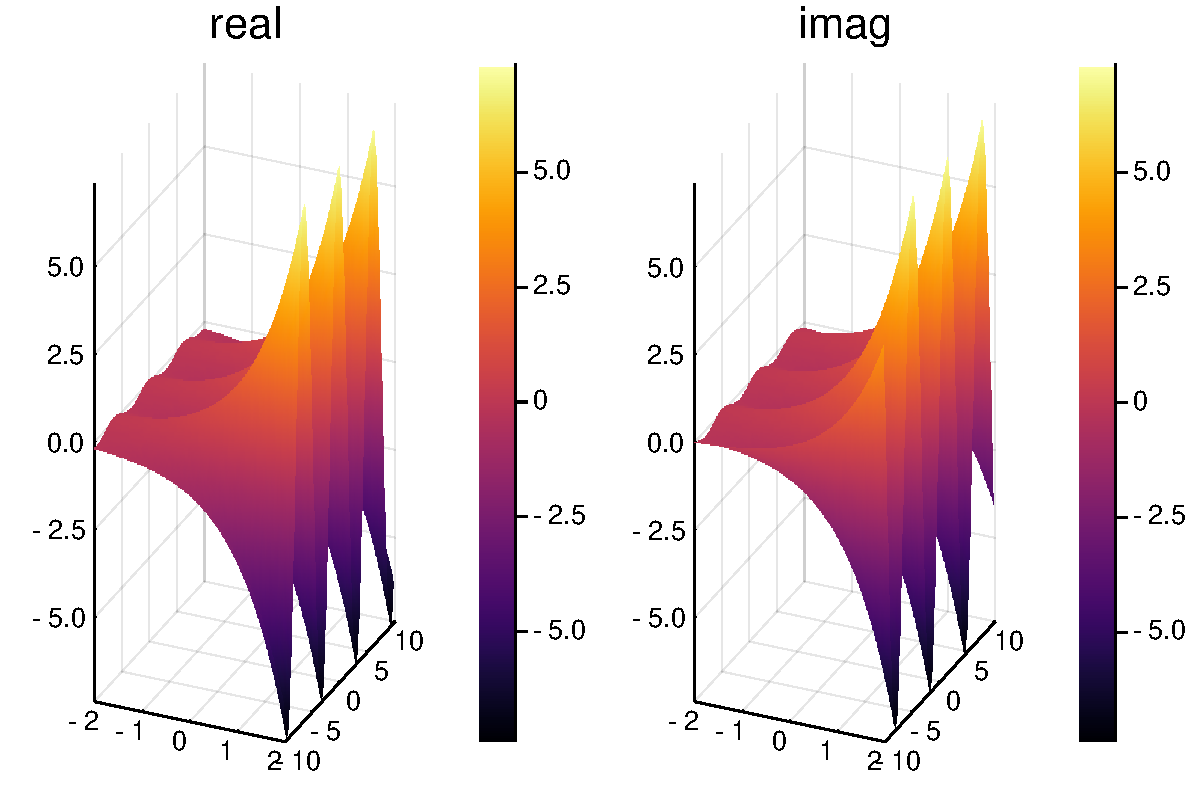
\includegraphics[width=\linewidth]{figures/Lecture1_1_1.pdf}

Or a heat plot:


\begin{lstlisting}
(*@\HLJLnf{plot}@*)(*@\HLJLp{(}@*)(*@\HLJLnf{contourf}@*)(*@\HLJLp{(}@*)(*@\HLJLn{xx}@*)(*@\HLJLp{,}@*) (*@\HLJLn{yy}@*)(*@\HLJLp{,}@*) (*@\HLJLn{u}@*)(*@\HLJLoB{.}@*)(*@\HLJLp{(}@*)(*@\HLJLn{xx}@*)(*@\HLJLoB{{\textquotesingle}}@*) (*@\HLJLoB{.+}@*) (*@\HLJLn{im}@*)(*@\HLJLoB{.*}@*)(*@\HLJLn{yy}@*)(*@\HLJLp{);}@*) (*@\HLJLn{title}@*)(*@\HLJLoB{=}@*)(*@\HLJLs{"{}real"{}}@*)(*@\HLJLp{),}@*)
     (*@\HLJLnf{contourf}@*)(*@\HLJLp{(}@*)(*@\HLJLn{xx}@*)(*@\HLJLp{,}@*) (*@\HLJLn{yy}@*)(*@\HLJLp{,}@*) (*@\HLJLn{v}@*)(*@\HLJLoB{.}@*)(*@\HLJLp{(}@*)(*@\HLJLn{xx}@*)(*@\HLJLoB{{\textquotesingle}}@*) (*@\HLJLoB{.+}@*) (*@\HLJLn{im}@*)(*@\HLJLoB{.*}@*)(*@\HLJLn{yy}@*)(*@\HLJLp{);}@*) (*@\HLJLn{title}@*)(*@\HLJLoB{=}@*)(*@\HLJLs{"{}imag"{}}@*)(*@\HLJLp{))}@*)
\end{lstlisting}

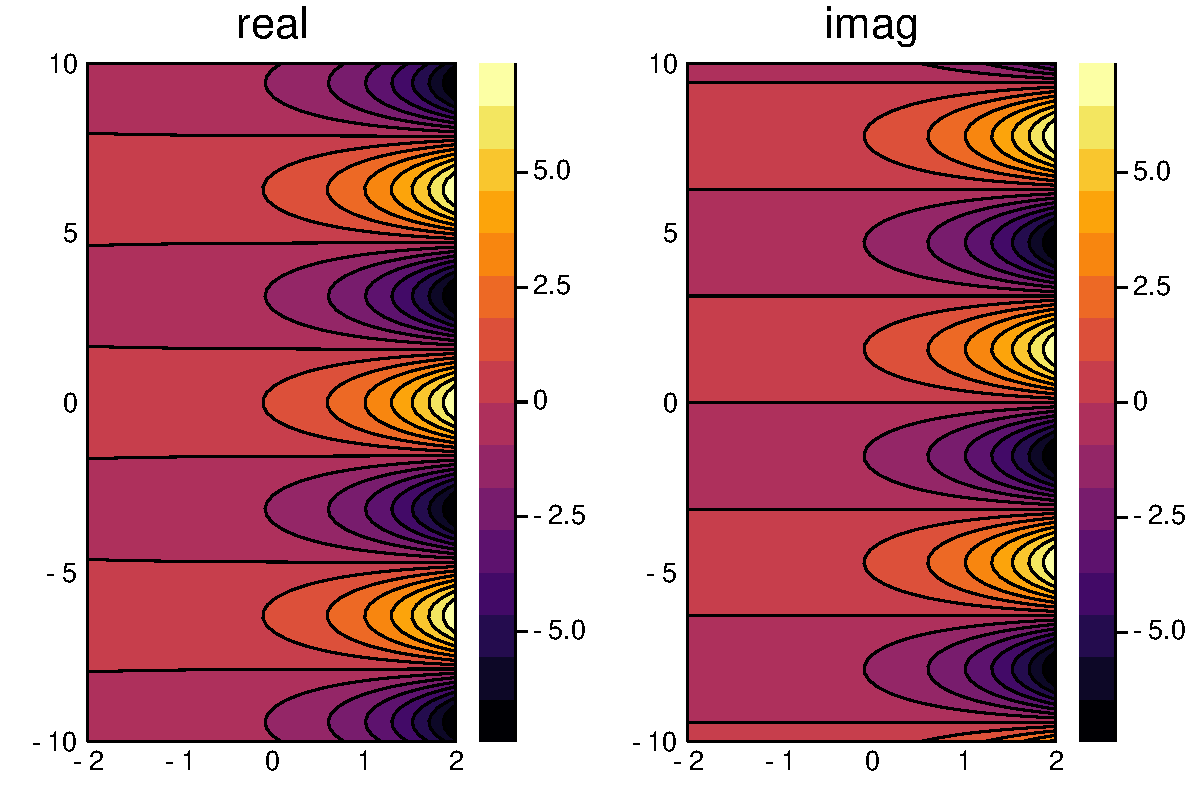
\includegraphics[width=\linewidth]{figures/Lecture1_2_1.pdf}

\textbf{Method 2: absolute-value and angle}

Every complex number $z$ can be written as $re^{i \theta}$ for $0 \leq r$ and $-\pi < \theta \leq \pi$. $r = |z|$ is called the \emph{absolute value} and $\theta$ is called the \emph{phase} or \emph{argument} (or in Julia, \emph{angle}).  We can plot these:


\begin{lstlisting}
(*@\HLJLn{xx}@*) (*@\HLJLoB{=}@*) (*@\HLJLoB{-}@*)(*@\HLJLni{2}@*)(*@\HLJLoB{:}@*)(*@\HLJLnfB{0.01}@*)(*@\HLJLoB{:}@*)(*@\HLJLni{2}@*)
(*@\HLJLn{yy}@*) (*@\HLJLoB{=}@*) (*@\HLJLoB{-}@*)(*@\HLJLni{10}@*)(*@\HLJLoB{:}@*)(*@\HLJLnfB{0.01}@*)(*@\HLJLoB{:}@*)(*@\HLJLni{10}@*)

(*@\HLJLn{f}@*) (*@\HLJLoB{=}@*) (*@\HLJLn{z}@*) (*@\HLJLoB{->}@*) (*@\HLJLnf{exp}@*)(*@\HLJLp{(}@*)(*@\HLJLn{z}@*)(*@\HLJLp{)}@*)

(*@\HLJLn{r}@*) (*@\HLJLoB{=}@*) (*@\HLJLn{z}@*) (*@\HLJLoB{->}@*) (*@\HLJLnf{abs}@*)(*@\HLJLp{(}@*)(*@\HLJLnf{f}@*)(*@\HLJLp{(}@*)(*@\HLJLn{z}@*)(*@\HLJLp{))}@*)
(*@\HLJLn{\ensuremath{\theta}}@*) (*@\HLJLoB{=}@*) (*@\HLJLn{z}@*) (*@\HLJLoB{->}@*) (*@\HLJLnf{angle}@*)(*@\HLJLp{(}@*)(*@\HLJLnf{f}@*)(*@\HLJLp{(}@*)(*@\HLJLn{z}@*)(*@\HLJLp{))}@*)


(*@\HLJLnf{plot}@*)(*@\HLJLp{(}@*) (*@\HLJLnf{contourf}@*)(*@\HLJLp{(}@*)(*@\HLJLn{xx}@*)(*@\HLJLp{,}@*) (*@\HLJLn{yy}@*)(*@\HLJLp{,}@*) (*@\HLJLn{r}@*)(*@\HLJLoB{.}@*)(*@\HLJLp{(}@*)(*@\HLJLn{xx}@*)(*@\HLJLoB{{\textquotesingle}}@*) (*@\HLJLoB{.+}@*) (*@\HLJLn{im}@*)(*@\HLJLoB{.*}@*)(*@\HLJLn{yy}@*)(*@\HLJLp{);}@*) (*@\HLJLn{title}@*)(*@\HLJLoB{=}@*)(*@\HLJLs{"{}abs"{}}@*)(*@\HLJLp{),}@*)
      (*@\HLJLnf{contourf}@*)(*@\HLJLp{(}@*)(*@\HLJLn{xx}@*)(*@\HLJLp{,}@*) (*@\HLJLn{yy}@*)(*@\HLJLp{,}@*) (*@\HLJLn{\ensuremath{\theta}}@*)(*@\HLJLoB{.}@*)(*@\HLJLp{(}@*)(*@\HLJLn{xx}@*)(*@\HLJLoB{{\textquotesingle}}@*) (*@\HLJLoB{.+}@*) (*@\HLJLn{im}@*)(*@\HLJLoB{.*}@*)(*@\HLJLn{yy}@*)(*@\HLJLp{);}@*) (*@\HLJLn{title}@*)(*@\HLJLoB{=}@*)(*@\HLJLs{"{}phase"{}}@*)(*@\HLJLp{))}@*)
\end{lstlisting}

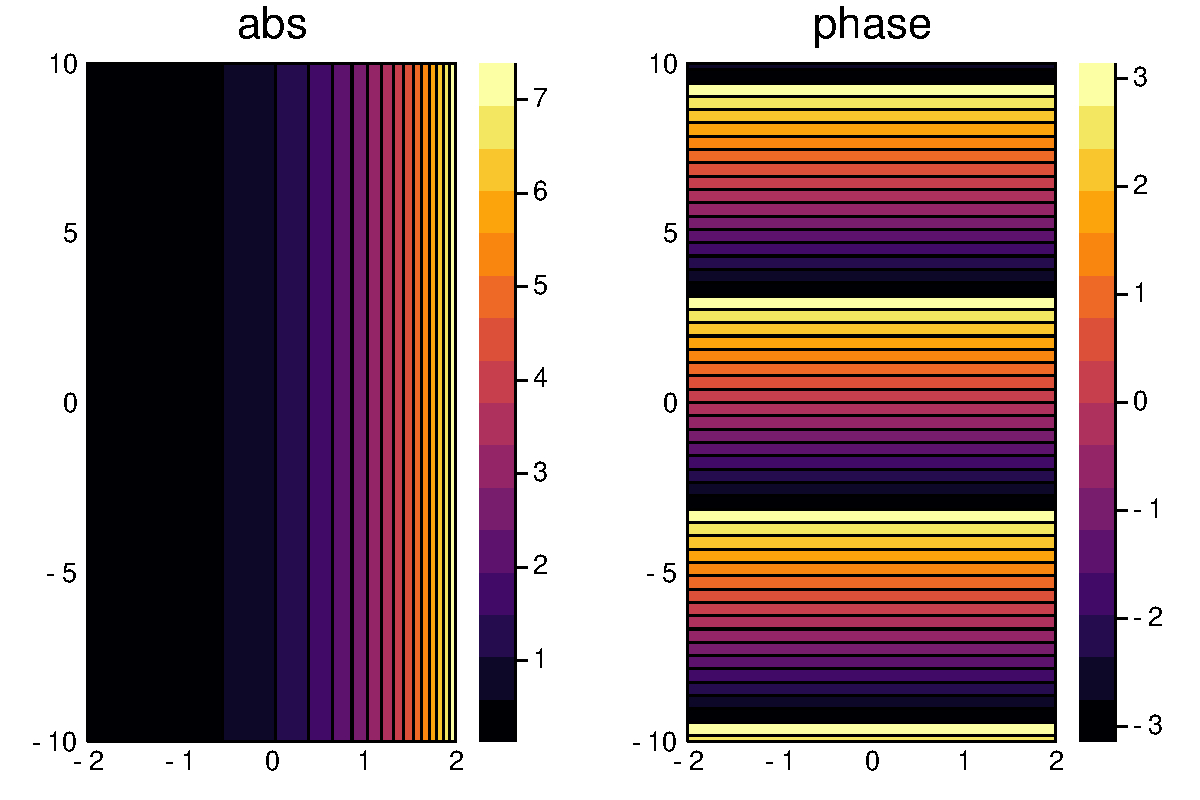
\includegraphics[width=\linewidth]{figures/Lecture1_3_1.pdf}

\_\_ Method 3: Phase portrait \_\_

This method is essentially the same, as before, but to \emph{only} plot the phase, and use a "colour wheel" to reflect the topology of $\theta$. 


\begin{lstlisting}
(*@\HLJLnf{phaseplot}@*)(*@\HLJLp{(}@*)(*@\HLJLoB{-}@*)(*@\HLJLnfB{3..3}@*)(*@\HLJLp{,}@*) (*@\HLJLoB{-}@*)(*@\HLJLnfB{8..8}@*)(*@\HLJLp{,}@*) (*@\HLJLn{z}@*) (*@\HLJLoB{->}@*) (*@\HLJLnf{exp}@*)(*@\HLJLp{(}@*)(*@\HLJLn{z}@*)(*@\HLJLp{))}@*)
\end{lstlisting}

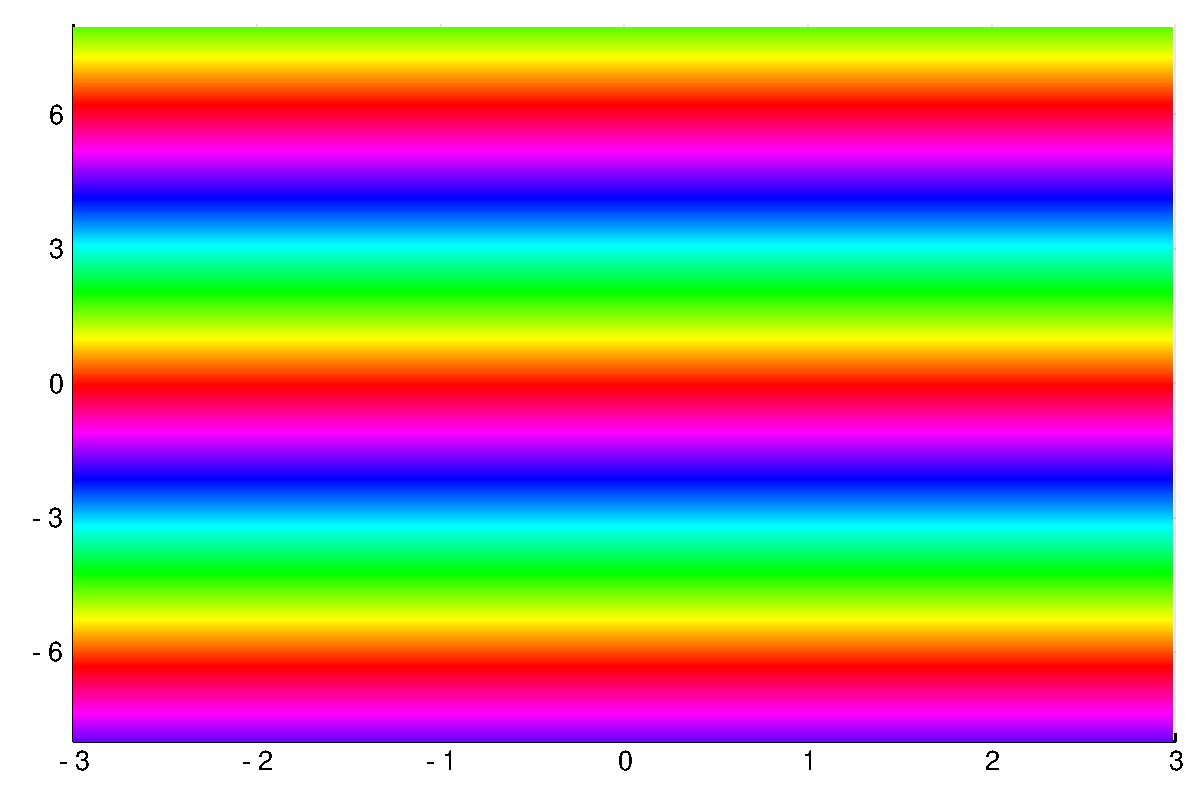
\includegraphics[width=\linewidth]{figures/Lecture1_4_1.pdf}

This is seen most clearly with $f(z) = z$: in this case, letting $z = r \E^{\I \theta}$ we are simply plotting $\theta$:


\begin{lstlisting}
(*@\HLJLnf{phaseplot}@*)(*@\HLJLp{(}@*)(*@\HLJLoB{-}@*)(*@\HLJLnfB{3..3}@*)(*@\HLJLp{,}@*) (*@\HLJLoB{-}@*)(*@\HLJLnfB{3..3}@*)(*@\HLJLp{,}@*) (*@\HLJLn{z}@*) (*@\HLJLoB{->}@*) (*@\HLJLn{z}@*)(*@\HLJLp{)}@*)
\end{lstlisting}

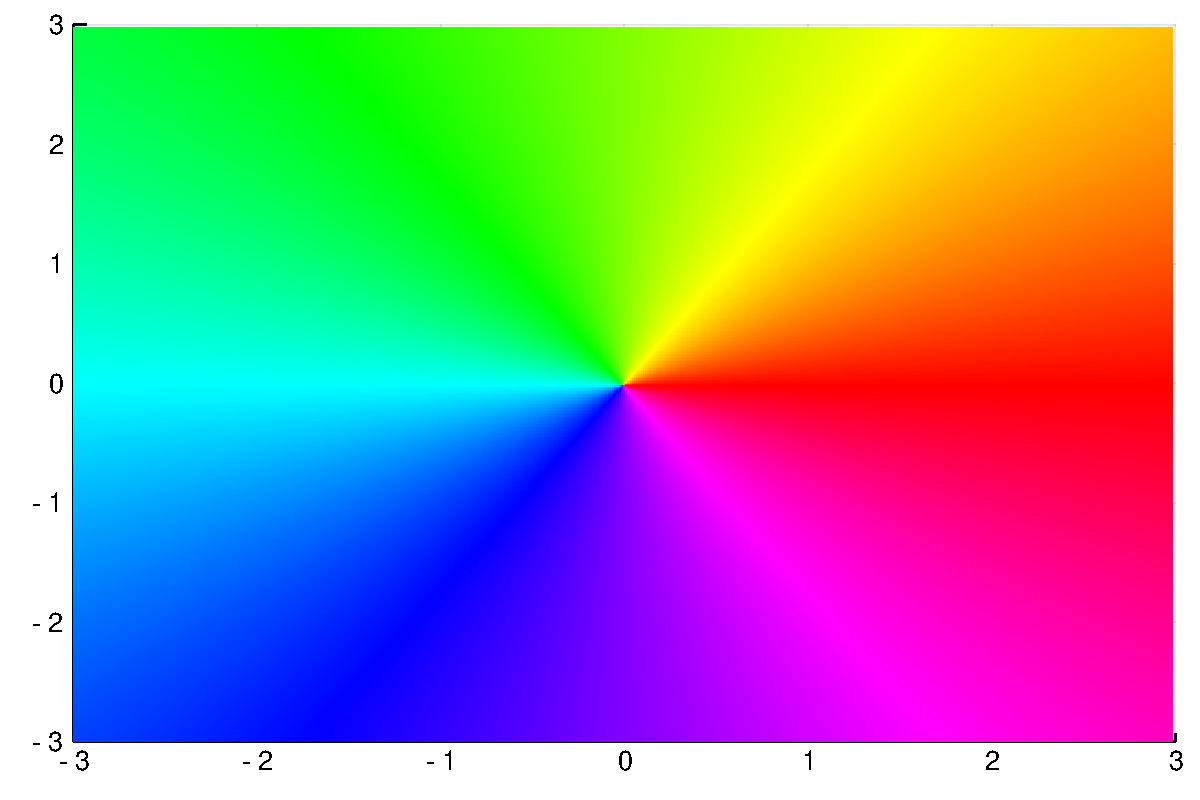
\includegraphics[width=\linewidth]{figures/Lecture1_5_1.pdf}

In other words, the colour red corresponds to $\arg f(z) \approx 0$, green to $\arg f(z) \approx {2 \pi \over 3}$ aqua to $\arg f(z) \approx \pi$ and so on. 

Note that multiplying $z$ by a complex number $R \E^{\I \varphi}$ will rotate the wheel, but the colours still appear in the same order when read counter clockwise:


\begin{lstlisting}
(*@\HLJLnf{phaseplot}@*)(*@\HLJLp{(}@*)(*@\HLJLoB{-}@*)(*@\HLJLnfB{3..3}@*)(*@\HLJLp{,}@*) (*@\HLJLoB{-}@*)(*@\HLJLnfB{3..3}@*)(*@\HLJLp{,}@*) (*@\HLJLn{z}@*) (*@\HLJLoB{->}@*) (*@\HLJLnf{exp}@*)(*@\HLJLp{(}@*)(*@\HLJLnfB{1.0}@*)(*@\HLJLn{im}@*)(*@\HLJLp{)}@*)(*@\HLJLoB{*}@*)(*@\HLJLn{z}@*)(*@\HLJLp{)}@*)
\end{lstlisting}

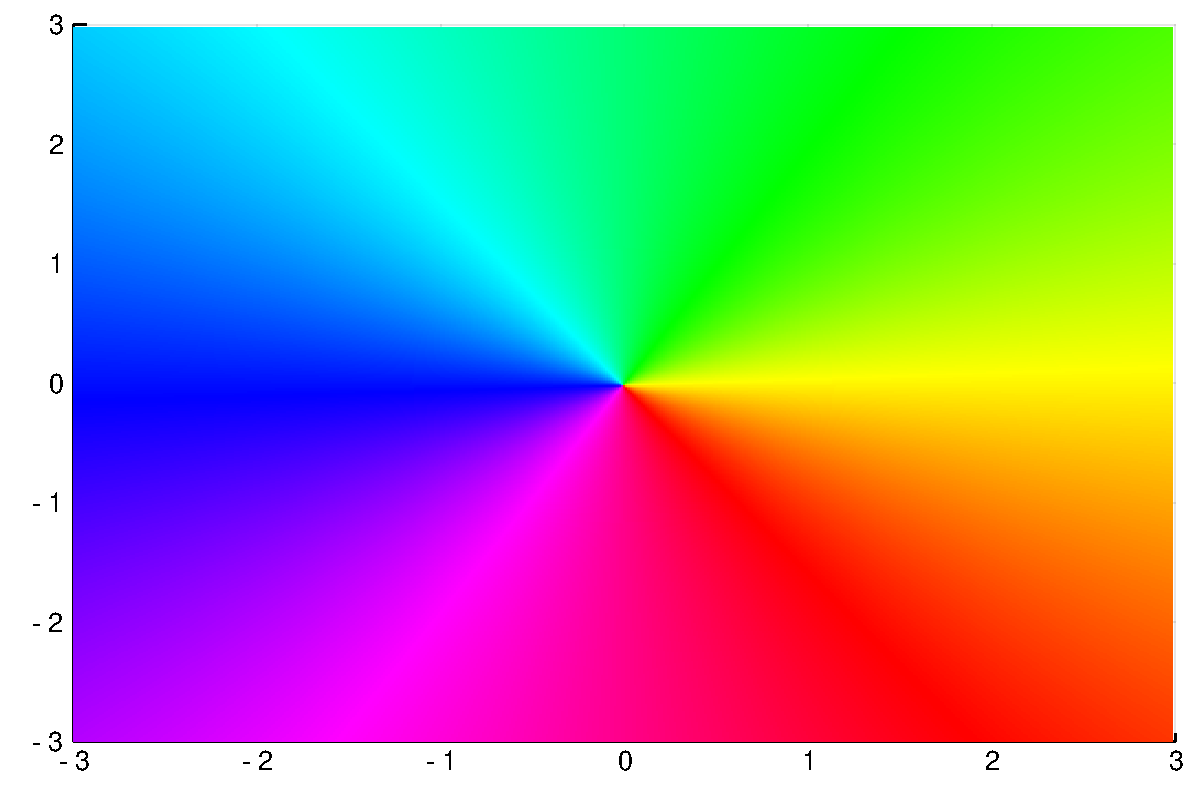
\includegraphics[width=\linewidth]{figures/Lecture1_6_1.pdf}

Therefore, if $f(z)$ has a zero at $z_0$, since it behaves like $f(z) = f'(z_0) (z - z_0)$, we will have the full colour wheel always in the counter clockwise order red\ensuremath{\endash}green\ensuremath{\endash}blue\ensuremath{\endash}red:


\begin{lstlisting}
(*@\HLJLnf{phaseplot}@*)(*@\HLJLp{(}@*)(*@\HLJLoB{-}@*)(*@\HLJLnfB{20..20}@*)(*@\HLJLp{,}@*) (*@\HLJLoB{-}@*)(*@\HLJLnfB{3..3}@*)(*@\HLJLp{,}@*) (*@\HLJLn{z}@*) (*@\HLJLoB{->}@*) (*@\HLJLnf{sin}@*)(*@\HLJLp{(}@*)(*@\HLJLn{z}@*)(*@\HLJLp{))}@*)
\end{lstlisting}

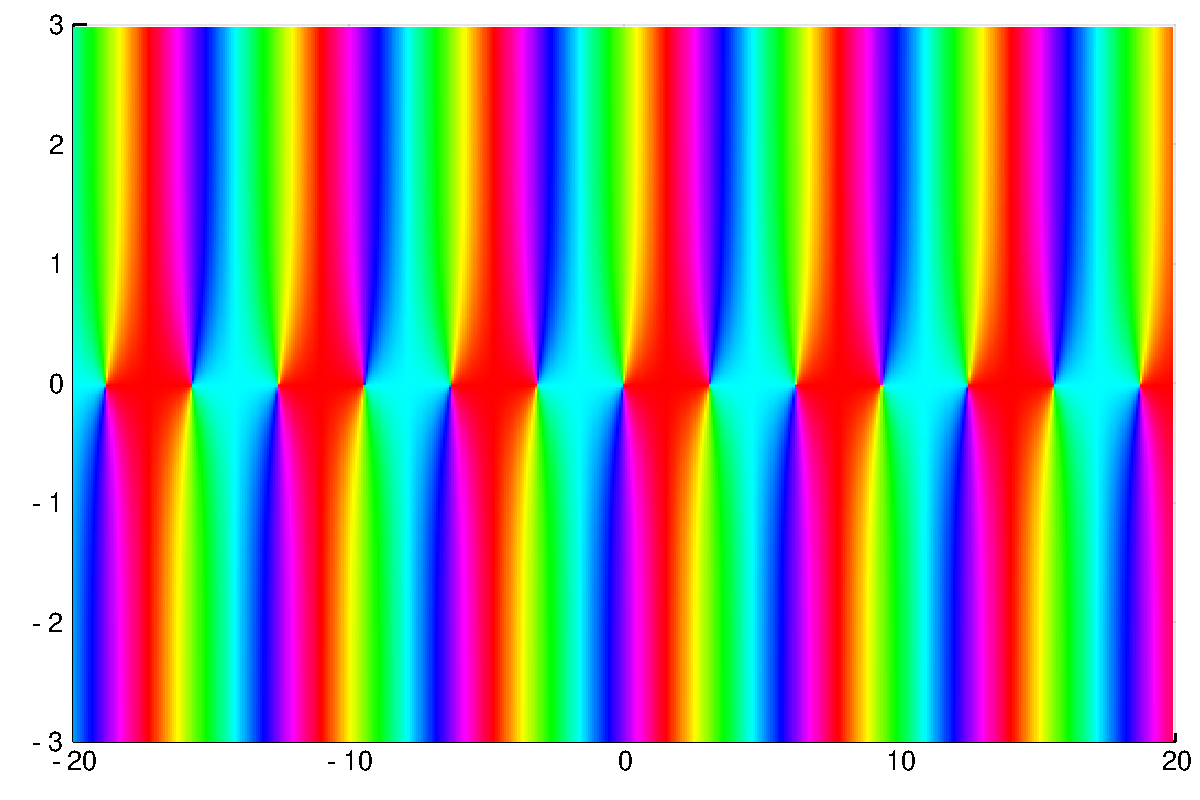
\includegraphics[width=\linewidth]{figures/Lecture1_7_1.pdf}

In the case of a double root like $f(z) = z^2 = r \E^{2 \I \theta}$, we have the wheel appearing twice, but still in the same order. Thus the order of a zero can be seen by the number of times we go around the colour wheel: here we see that the function has a triple root at zero since it goes red\ensuremath{\endash}green\ensuremath{\endash}blue\ensuremath{\endash}red\ensuremath{\endash}green\ensuremath{\endash}blue\ensuremath{\endash}red\ensuremath{\endash}green\ensuremath{\endash}blue\ensuremath{\endash}red:


\begin{lstlisting}
(*@\HLJLnf{phaseplot}@*)(*@\HLJLp{(}@*)(*@\HLJLoB{-}@*)(*@\HLJLnfB{5..5}@*)(*@\HLJLp{,}@*) (*@\HLJLoB{-}@*)(*@\HLJLnfB{3..3}@*)(*@\HLJLp{,}@*) (*@\HLJLn{z}@*) (*@\HLJLoB{->}@*) (*@\HLJLn{z}@*)(*@\HLJLoB{{\textasciicircum}}@*)(*@\HLJLni{2}@*)(*@\HLJLoB{*}@*)(*@\HLJLnf{sin}@*)(*@\HLJLp{(}@*)(*@\HLJLn{z}@*)(*@\HLJLp{))}@*)
\end{lstlisting}

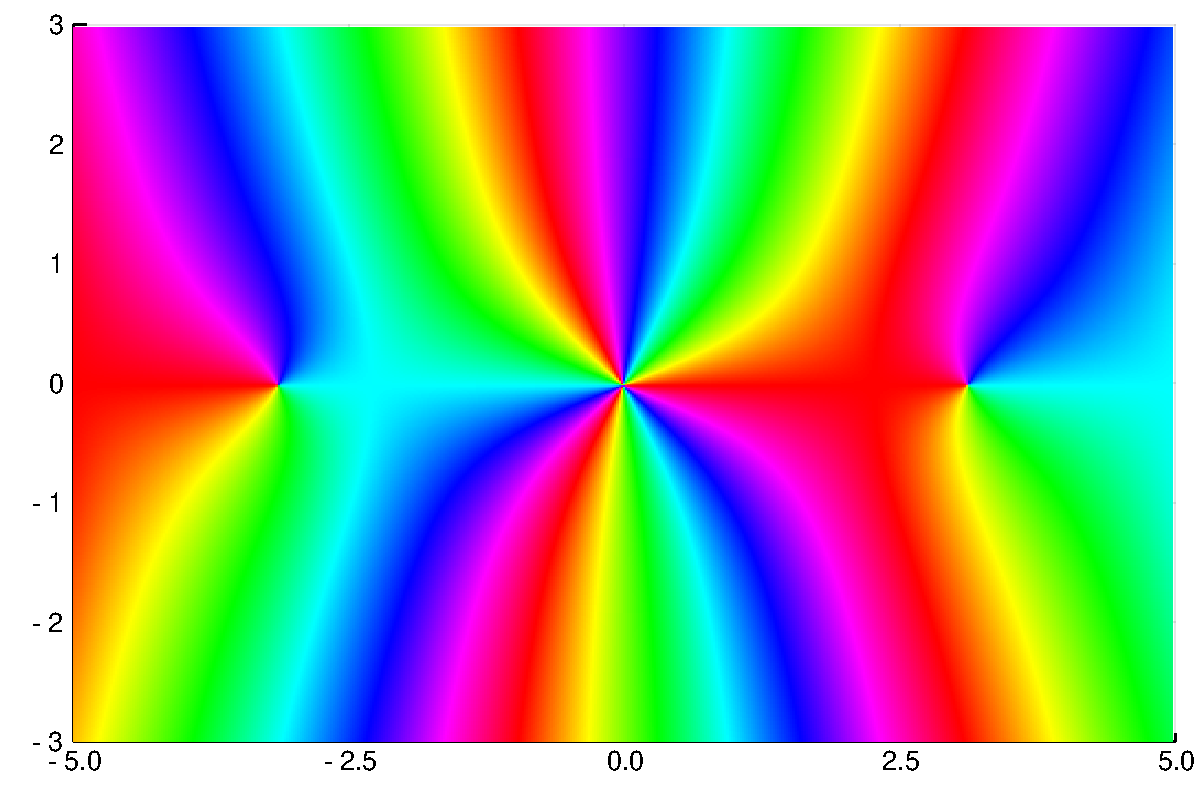
\includegraphics[width=\linewidth]{figures/Lecture1_8_1.pdf}

On the other hand, if we plot $f(z) = z^{-1} = r^{-1} \E^{-\I \theta}$ the wheel is reversed to  be red\ensuremath{\endash}blue\ensuremath{\endash}green\ensuremath{\endash}red:


\begin{lstlisting}
(*@\HLJLnf{phaseplot}@*)(*@\HLJLp{(}@*)(*@\HLJLoB{-}@*)(*@\HLJLnfB{3..3}@*)(*@\HLJLp{,}@*) (*@\HLJLoB{-}@*)(*@\HLJLnfB{3..3}@*)(*@\HLJLp{,}@*) (*@\HLJLn{z}@*) (*@\HLJLoB{->}@*) (*@\HLJLni{1}@*)(*@\HLJLoB{/}@*)(*@\HLJLn{z}@*)(*@\HLJLp{)}@*)
\end{lstlisting}

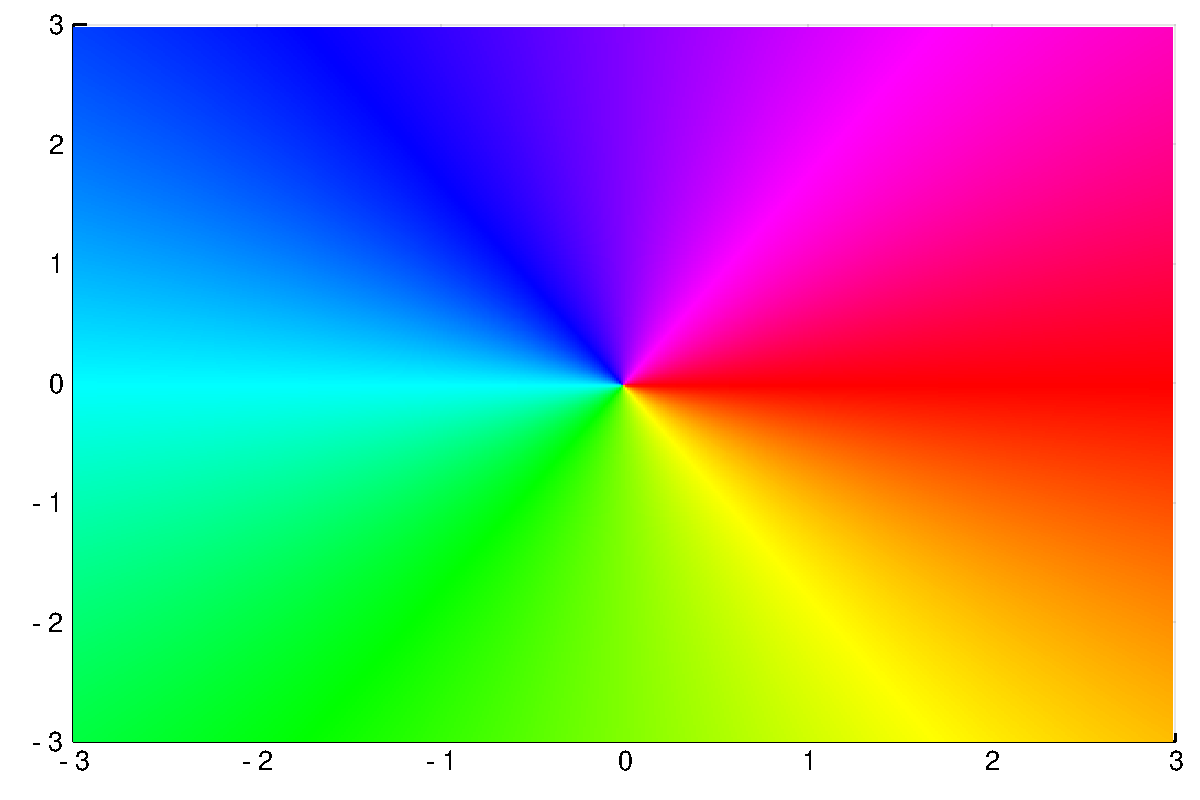
\includegraphics[width=\linewidth]{figures/Lecture1_9_1.pdf}

Thus we can see from a phase plot where the poles and zeros are, and the order of the poles and roots: the following function has a double pole at 0 (red\ensuremath{\endash}blue\ensuremath{\endash}green\ensuremath{\endash}red\ensuremath{\endash}blue\ensuremath{\endash}green), a zero at $-{\pi \over 2}$ (red\ensuremath{\endash}green\ensuremath{\endash}blue\ensuremath{\endash}red) and a double zero at $\pi\over 2$ (red\ensuremath{\endash}green\ensuremath{\endash}blue\ensuremath{\endash}red\ensuremath{\endash}green\ensuremath{\endash}blue\ensuremath{\endash}red) :


\begin{lstlisting}
(*@\HLJLnf{phaseplot}@*)(*@\HLJLp{(}@*) (*@\HLJLoB{-}@*)(*@\HLJLnfB{3..5}@*)(*@\HLJLp{,}@*) (*@\HLJLoB{-}@*)(*@\HLJLnfB{3..3}@*)(*@\HLJLp{,}@*) (*@\HLJLn{z}@*) (*@\HLJLoB{->}@*) (*@\HLJLnf{cot}@*)(*@\HLJLp{(}@*)(*@\HLJLn{z}@*)(*@\HLJLp{)}@*)(*@\HLJLoB{/}@*)(*@\HLJLn{z}@*)(*@\HLJLoB{*}@*)(*@\HLJLp{(}@*)(*@\HLJLn{\ensuremath{\pi}}@*)(*@\HLJLoB{/}@*)(*@\HLJLni{2}@*)(*@\HLJLoB{-}@*)(*@\HLJLn{z}@*)(*@\HLJLp{))}@*)
\end{lstlisting}

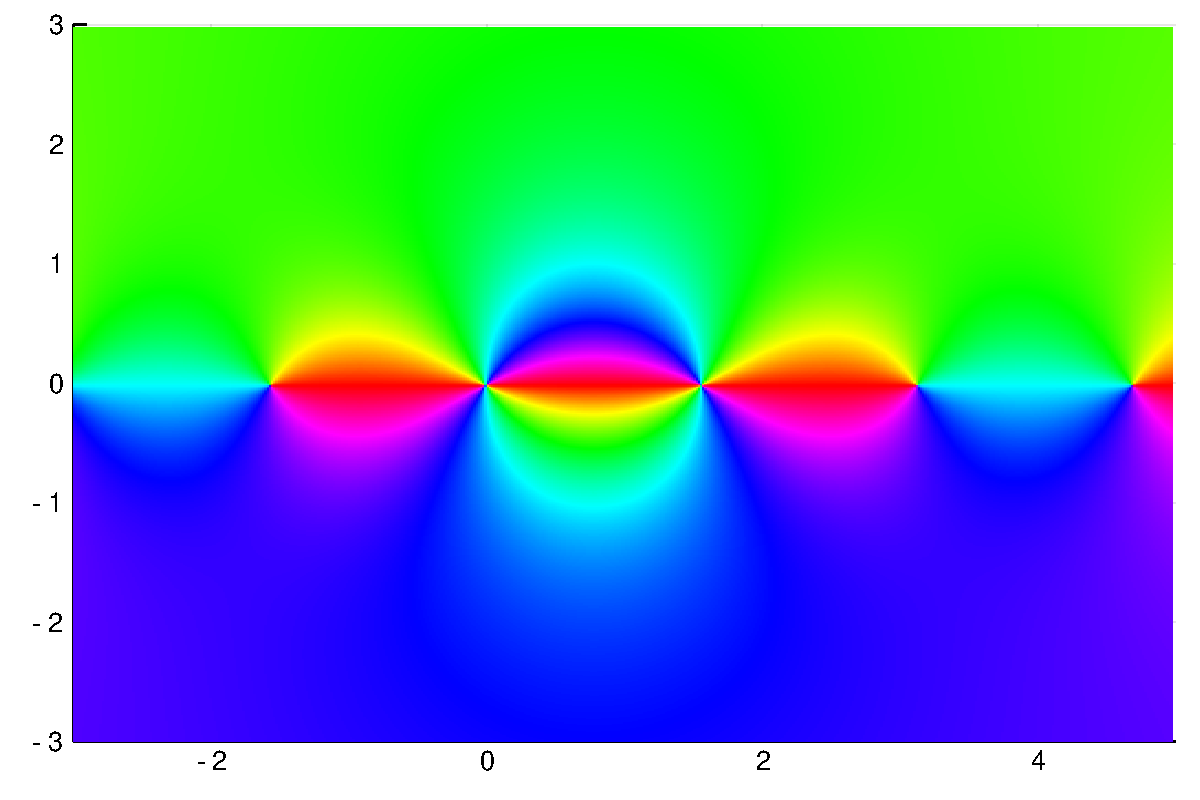
\includegraphics[width=\linewidth]{figures/Lecture1_10_1.pdf}

Functions with more complicated singularities do not have such nice phase plots (these are what we will call \emph{essential} singularities):


\begin{lstlisting}
(*@\HLJLnf{phaseplot}@*)(*@\HLJLp{(}@*)(*@\HLJLoB{-}@*)(*@\HLJLnfB{3..3}@*)(*@\HLJLp{,}@*) (*@\HLJLoB{-}@*)(*@\HLJLnfB{3..3}@*)(*@\HLJLp{,}@*) (*@\HLJLn{z}@*) (*@\HLJLoB{->}@*) (*@\HLJLnf{exp}@*)(*@\HLJLp{(}@*)(*@\HLJLni{1}@*)(*@\HLJLoB{/}@*)(*@\HLJLn{z}@*)(*@\HLJLp{))}@*)
\end{lstlisting}

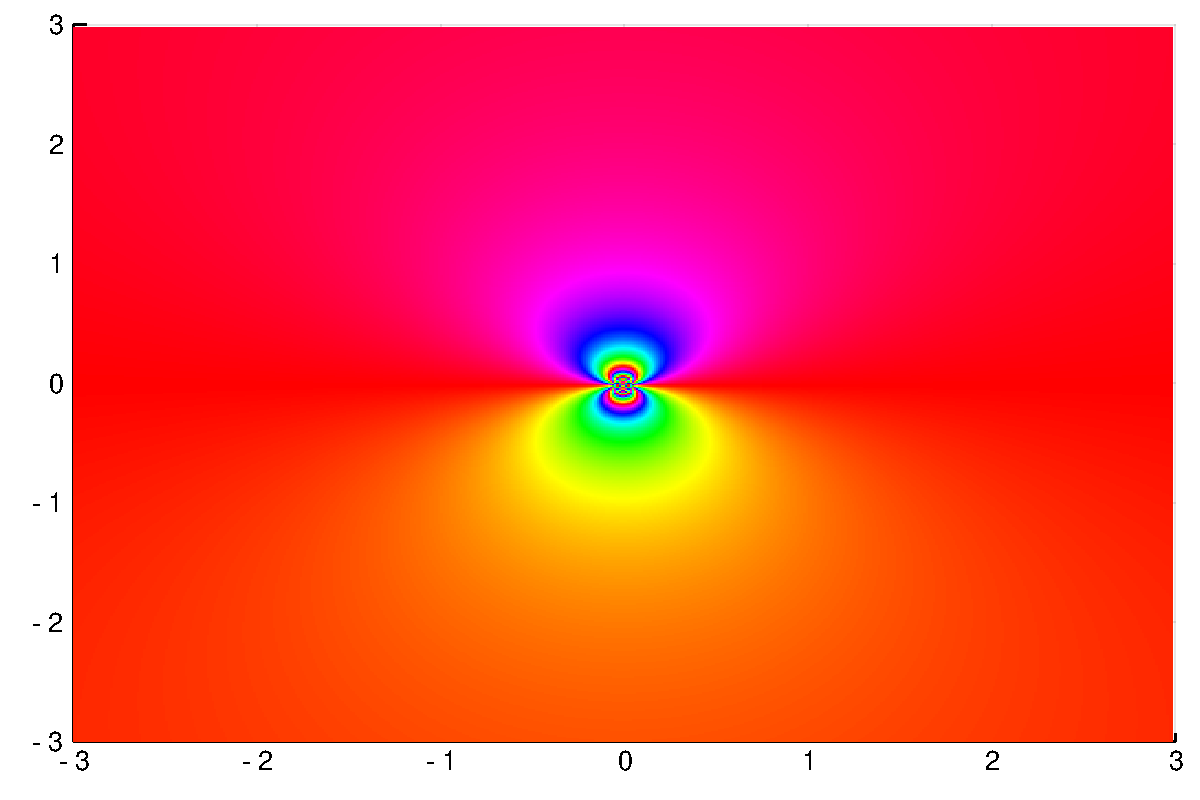
\includegraphics[width=\linewidth]{figures/Lecture1_11_1.pdf}

The jumps of functions like $\log z$ or $\sqrt z$ also appear naturally in the phase plot: here we see $\log z$ has a zero at $1$ (red\ensuremath{\endash}green\ensuremath{\endash}blue\ensuremath{\endash}red) and a jump along $(-\infty,0]$


\begin{lstlisting}
(*@\HLJLnf{phaseplot}@*)(*@\HLJLp{(}@*) (*@\HLJLoB{-}@*)(*@\HLJLnfB{3..3}@*)(*@\HLJLp{,}@*) (*@\HLJLoB{-}@*)(*@\HLJLnfB{3..3}@*)(*@\HLJLp{,}@*) (*@\HLJLn{z}@*) (*@\HLJLoB{->}@*) (*@\HLJLnf{log}@*)(*@\HLJLp{(}@*)(*@\HLJLn{z}@*)(*@\HLJLp{))}@*)
\end{lstlisting}

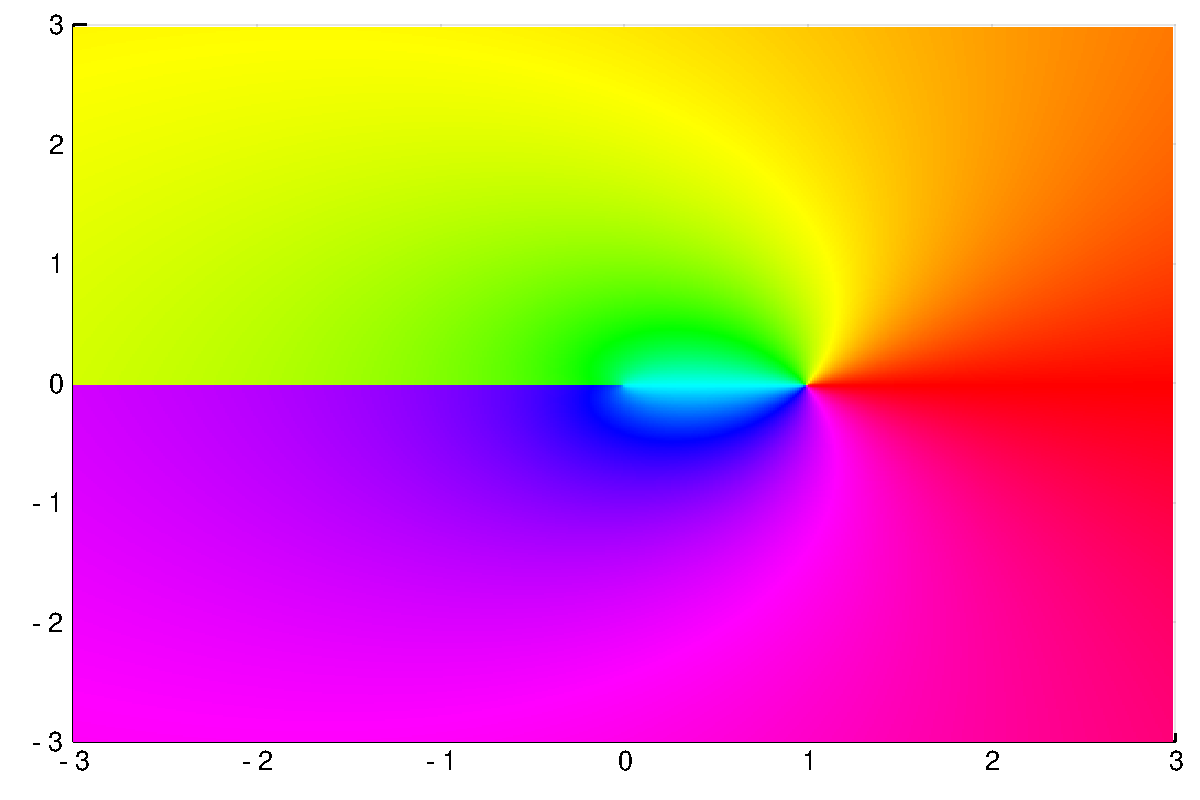
\includegraphics[width=\linewidth]{figures/Lecture1_12_1.pdf}

Often, singularities are in the complex plane. can you determine where the zeros and roots, and their orders, of the following function are from the picture?


\begin{lstlisting}
(*@\HLJLnf{phaseplot}@*)(*@\HLJLp{(}@*)(*@\HLJLoB{-}@*)(*@\HLJLnfB{3..3}@*)(*@\HLJLp{,}@*) (*@\HLJLoB{-}@*)(*@\HLJLnfB{3..3}@*)(*@\HLJLp{,}@*) (*@\HLJLn{z}@*) (*@\HLJLoB{->}@*) (*@\HLJLn{z}@*)(*@\HLJLoB{{\textasciicircum}}@*)(*@\HLJLni{5}@*)  (*@\HLJLoB{/}@*) (*@\HLJLp{(}@*)(*@\HLJLni{1}@*) (*@\HLJLoB{+}@*) (*@\HLJLn{z}@*)(*@\HLJLoB{{\textasciicircum}}@*)(*@\HLJLni{2}@*)(*@\HLJLp{)}@*)(*@\HLJLoB{{\textasciicircum}}@*)(*@\HLJLni{3}@*)(*@\HLJLp{)}@*)
\end{lstlisting}

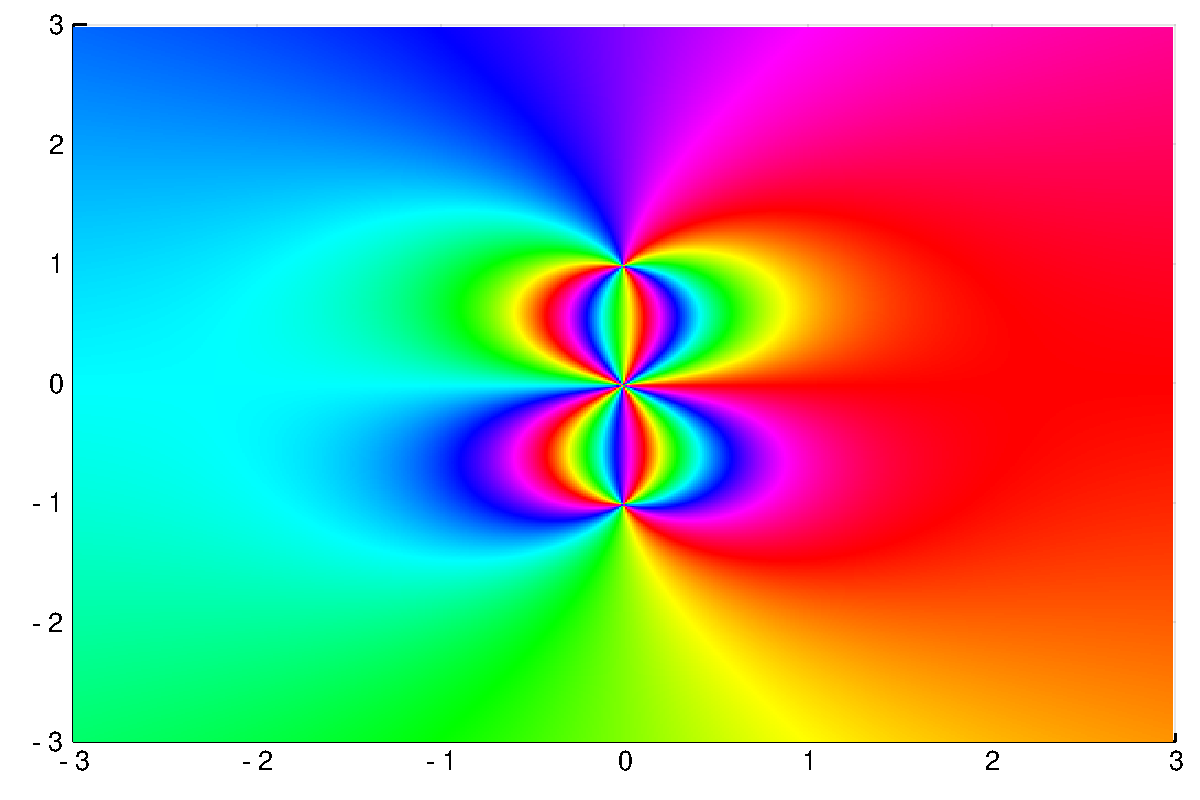
\includegraphics[width=\linewidth]{figures/Lecture1_13_1.pdf}

\begin{lstlisting}
(*@\HLJLnf{phaseplot}@*)(*@\HLJLp{(}@*)(*@\HLJLoB{-}@*)(*@\HLJLnfB{3..3}@*)(*@\HLJLp{,}@*) (*@\HLJLoB{-}@*)(*@\HLJLnfB{3..3}@*)(*@\HLJLp{,}@*) (*@\HLJLn{z}@*) (*@\HLJLoB{->}@*) (*@\HLJLnf{erfc}@*)(*@\HLJLp{(}@*)(*@\HLJLn{z}@*)(*@\HLJLp{))}@*)
\end{lstlisting}

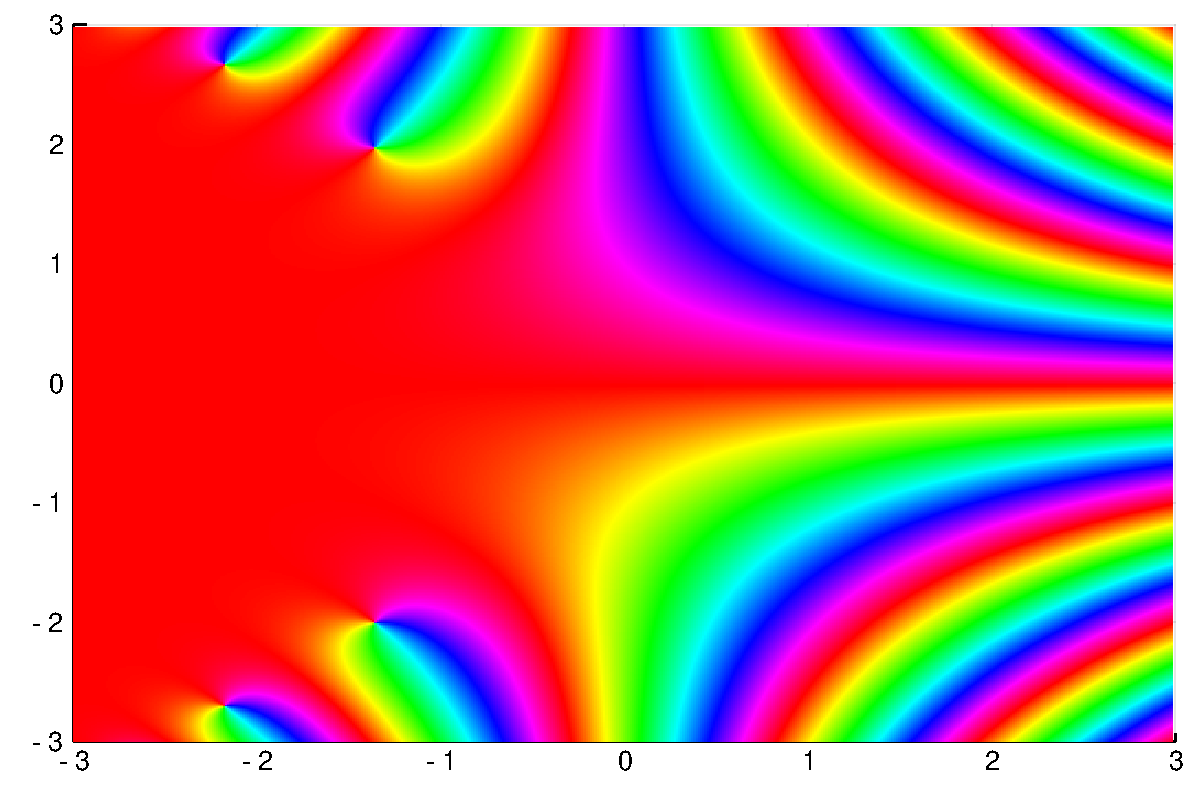
\includegraphics[width=\linewidth]{figures/Lecture1_14_1.pdf}

Here's the Gamma function. Are they poles or zeros at 0, -1, -2, ...?


\begin{lstlisting}
(*@\HLJLnf{phaseplot}@*)(*@\HLJLp{(}@*)(*@\HLJLoB{-}@*)(*@\HLJLnfB{3..3}@*)(*@\HLJLp{,}@*) (*@\HLJLoB{-}@*)(*@\HLJLnfB{3..3}@*)(*@\HLJLp{,}@*) (*@\HLJLn{z}@*) (*@\HLJLoB{->}@*) (*@\HLJLnf{gamma}@*)(*@\HLJLp{(}@*)(*@\HLJLn{z}@*)(*@\HLJLp{))}@*)
\end{lstlisting}

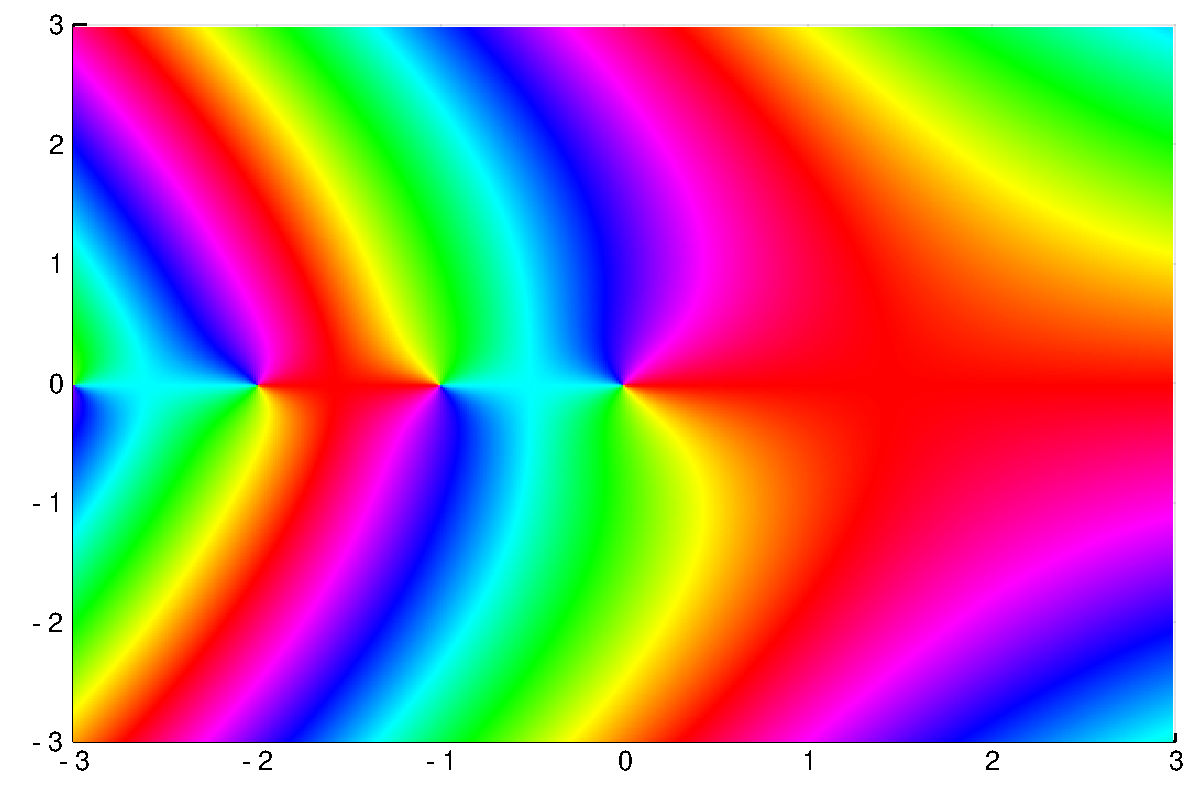
\includegraphics[width=\linewidth]{figures/Lecture1_15_1.pdf}

Something strange is happening at -1/2, -3/2, .... What if we differentiate? Here \texttt{dual(z,1)} is a \href{https://en.wikipedia.org/wiki/Dual_number}{dual number}, which provides a convenient way to implement automatic differentiation: \texttt{gammap(z)} is derivative of \texttt{gamma(z)} w.r.t. \texttt{z}.


\begin{lstlisting}
(*@\HLJLk{using}@*) (*@\HLJLn{DualNumbers}@*)
(*@\HLJLn{gammap}@*) (*@\HLJLoB{=}@*) (*@\HLJLn{z}@*) (*@\HLJLoB{->}@*) (*@\HLJLnf{epsilon}@*)(*@\HLJLp{(}@*)(*@\HLJLnf{gamma}@*)(*@\HLJLp{(}@*)(*@\HLJLnf{dual}@*)(*@\HLJLp{(}@*)(*@\HLJLn{z}@*)(*@\HLJLp{,}@*)(*@\HLJLni{1}@*)(*@\HLJLp{)))}@*)
(*@\HLJLnf{phaseplot}@*)(*@\HLJLp{(}@*)(*@\HLJLoB{-}@*)(*@\HLJLnfB{3..3}@*)(*@\HLJLp{,}@*) (*@\HLJLoB{-}@*)(*@\HLJLnfB{3..3}@*)(*@\HLJLp{,}@*) (*@\HLJLn{gammap}@*)(*@\HLJLp{)}@*)
\end{lstlisting}

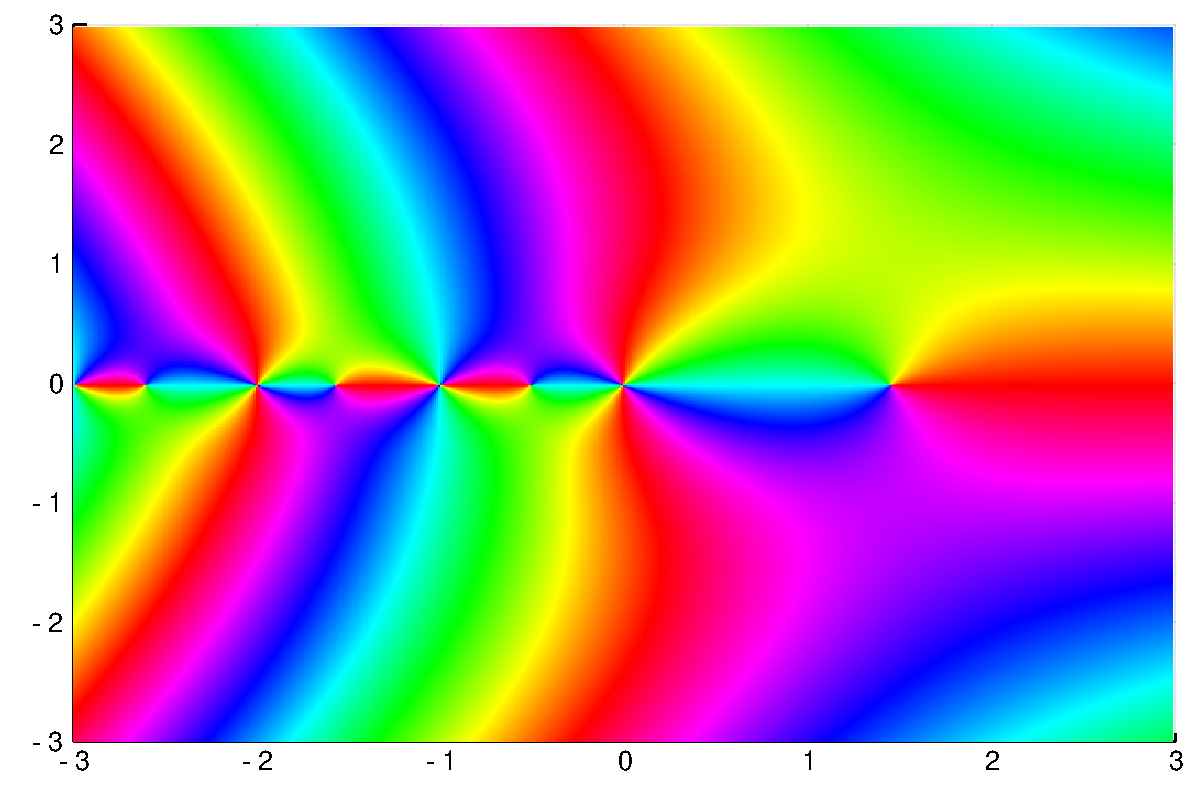
\includegraphics[width=\linewidth]{figures/Lecture1_16_1.pdf}

Finally, the Riemann Hypothesis: Here is a plot of the Riemann zeta function near the critical line $z = 0.5 + \I t$:


\begin{lstlisting}
(*@\HLJLnf{phaseplot}@*)(*@\HLJLp{(}@*)(*@\HLJLni{0}@*)(*@\HLJLoB{:}@*)(*@\HLJLnfB{0.011}@*)(*@\HLJLoB{:}@*)(*@\HLJLni{2}@*)(*@\HLJLp{,}@*) (*@\HLJLoB{-}@*)(*@\HLJLni{2}@*)(*@\HLJLoB{:}@*)(*@\HLJLnfB{0.011}@*)(*@\HLJLoB{:}@*)(*@\HLJLni{40}@*)(*@\HLJLp{,}@*) (*@\HLJLn{zeta}@*)(*@\HLJLp{)}@*)
\end{lstlisting}

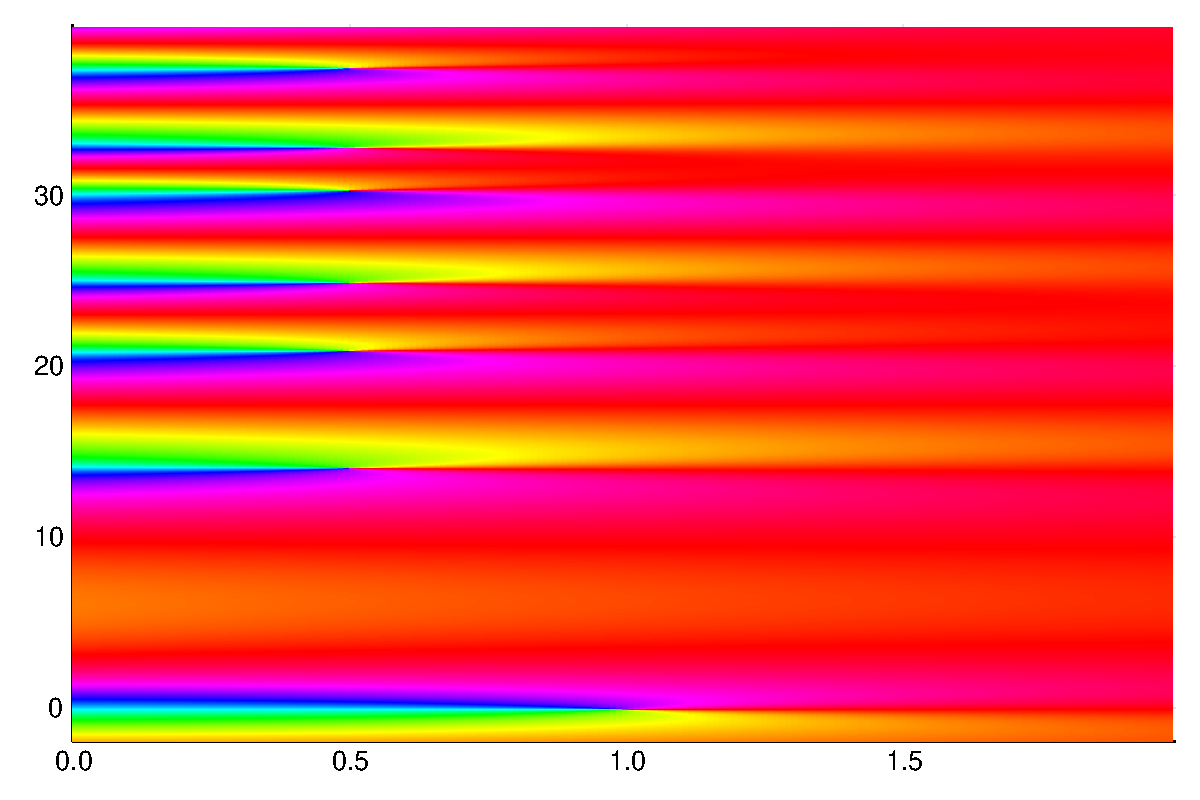
\includegraphics[width=\linewidth]{figures/Lecture1_17_1.pdf}

\subsection{Holomorphicity, Cauchy's theorem, and Analyticity}
A beautiful feature of complex analysis is one starts with a very weak assumption of holomorphicity, essentially complex-differentiability in an open set, deduce Cauchy's theorem and Cauchy's integral formula, which then imply analyticity. That is, if we assume a function is one-time complex differentiable, then it has an infinite number of derivatives.

These results are built up as follows:

\begin{itemize}
\item[1. ] Holomorphic functions


\item[2. ] Cauchy's theorem 


\item[3. ] Deformation of contours


\item[4. ] Cauchy's integral formula


\item[5. ] Analyticity and Taylor series

\end{itemize}
We will review the first three topics this lecture, with the remaining for next lecture.

\subsubsection{Holomorphic functions}
\textbf{Definition (Complex-differentiable)} Let $D \subset {\mathbb C}$ be an open set.  A function $f : D \rightarrow {\mathbb C}$ is called \emph{complex-differentiable} at a point $z_0 \in D$ if 

\[
   f'(z_0) =  \lim_{z \rightarrow z_0} {f(z) - f(z_0) \over z - z_0}
\]
exists, for any angle of approach to $z_0$.

\textbf{Definition (Holomorphic)} Let $D \subset {\mathbb C}$ be an open set.  A function $f : D \rightarrow {\mathbb C}$ is called \emph{holomorphic} in $D$ if it is complex-differentiable at all $z \in D$.

\textbf{Definition (Entire)} A function is \emph{entire} if it is holomorphic in ${\mathbb C}$

\emph{Examples}

\begin{itemize}
\item[1. ] \[
1
\]
is entire


\item[2. ] \[
z
\]
is entire


\item[3. ] \[
1/z
\]
is holomorphic in ${\mathbb C} \backslash \{0\}$


\item[4. ] \[
\sin z
\]
is entire


\item[5. ] \[
\csc z
\]
is holomorphic in ${\mathbb C} \backslash \{\ldots,-2\pi,-\pi,0,\pi,2\pi,\ldots\}$


\item[6. ] \[
\sqrt z
\]
is holomorphic in ${\mathbb C} \backslash (-\infty,0]$

\end{itemize}
\subsubsection{Cauchy's theorem}
\textbf{Definition (Contour)} A \emph{contour}  is a continuous \& piecewise-continuously differentiable function $\gamma : [a,b] \rightarrow {\mathbb C}$.

\textbf{Definition (Simple)} A \emph{simple contour} is a contour that is 1-to-1.

\textbf{Definition (Closed)} A \emph{closed contour} is a contour such that $\gamma(a) = \gamma(b)$

\emph{Examples of contours}

\begin{itemize}
\item[1. ] Line segment $[a,b]$ is a simple contour, with $\gamma(t) =  t$


\item[2. ] Arc from $re^{ia}$ to $re^{ib}$ is a simple contour, with $\gamma(t) =  re^{i t}$


\item[3. ] Circle of radius $r$ is a closed simple contour, with $\gamma(t) = re^{i t}$ and $a = -\pi$, $b = \pi$


\item[4. ] \[
\gamma(t) = \cos (t+i)^2
\]
defines a contour that is not simple or closed


\item[5. ] \[
\gamma(t) = e^{i t} + e^{2i t}
\]
for $[a,b] = [-\pi,\pi]$ defines a contour that is closed but not simple

\end{itemize}
\textbf{Definition (Contour integral)} The \emph{contour integral} over $\gamma$ is defined by

\[
\int_\gamma f(z) dz := \int_a^b f(\gamma(t)) \gamma'(t) dt
\]
An important property of a contour is its \emph{arclength}:

\textbf{Definition (Arclength)} The \emph{arclength} of $\gamma$ is defined as

\[
    {\cal L}(\gamma) := \int_a^b |\gamma'(t)| dt
\]
A very useful result is that we can use the maximum and arclength to bound integrals:

\textbf{Proposition (ML)} Let $f : \gamma \rightarrow {\mathbb C}$ and 

\[
        M = \sup_{z \in \gamma} |f(z)|
\]
Then

\[
\left|\int_\gamma f(z) dz \right| \leq M {\cal L}(\gamma)
\]
\textbf{Proposition} If $f(z)$ is holomorphic on $\gamma$, then $\int_\gamma f'(z) dz = f(\gamma(b)) - f(\gamma(a))$

\textbf{Theorem (Cauchy)} If $f$ is holomorphic inside and on a closed contour $\gamma$, then  $\oint_\gamma f(z) dz = 0$

\subsubsection{Deformation of contours}
\textbf{Definition (Domain)} A \emph{domain} is a non-empty, open and connected set $D \subset {\mathbb C}$.

\textbf{Definition (Homotopic)} Two closed contours $\gamma_1 : [a,b] \rightarrow D$ and $\gamma_2 \rightarrow D$ in a domain $D$ are \emph{homotopic} if they can be continuously deformed to one-another while remaining in $D$. 

\textbf{Theorem (Deformation of contours)} Let $f(z)$ be holomorphic in a domain $D$. Let $\gamma_1$ and $\gamma_2$ be two homotopic contours. Then

\[
    \int_{\gamma_1} f(z) dz = \int_{\gamma_2} f(z) dz
\]
\textbf{Definition (Simply connected)} A domain is \emph{simply connected} if every closed contour is homotoic to a point.

\textbf{Corollary (Deformation of contours on simply connected domains)} Let $f(z)$ be holomorphic in a simply-connected domain $D$. If $\gamma_1$ and $\gamma_2$ are two contours in $D$ with the same endpoints, then

\[
    \int_{\gamma_1} f(z) dz = \int_{\gamma_2} f(z) dz
\]
\subsubsection{Demonstration}
We can usually infer the domain where a function is holomorphic from a phase portrait, here we see that ${\rm arcsinh}\, z$ has cuts on $[\I,\I \infty)$ and $[-\I,-\I \infty)$, and a zero  (red\ensuremath{\endash}green\ensuremath{\endash}blue\ensuremath{\endash}red) at zero, hence we can infer that it is holomorphic in $\C \backslash ([\I,\I \infty) \cup [-\I,-\I \infty))$.


\begin{lstlisting}
(*@\HLJLk{using}@*) (*@\HLJLn{Plots}@*)(*@\HLJLp{,}@*) (*@\HLJLn{ComplexPhasePortrait}@*)(*@\HLJLp{,}@*) (*@\HLJLn{SpecialFunctions}@*)(*@\HLJLp{,}@*) (*@\HLJLn{ApproxFun}@*)
(*@\HLJLnf{phaseplot}@*)(*@\HLJLp{(}@*)(*@\HLJLoB{-}@*)(*@\HLJLnfB{4..4}@*)(*@\HLJLp{,}@*) (*@\HLJLoB{-}@*)(*@\HLJLnfB{4..4}@*)(*@\HLJLp{,}@*) (*@\HLJLn{z}@*) (*@\HLJLoB{->}@*) (*@\HLJLnf{asinh}@*)(*@\HLJLp{(}@*)(*@\HLJLn{z}@*)(*@\HLJLp{))}@*)
\end{lstlisting}

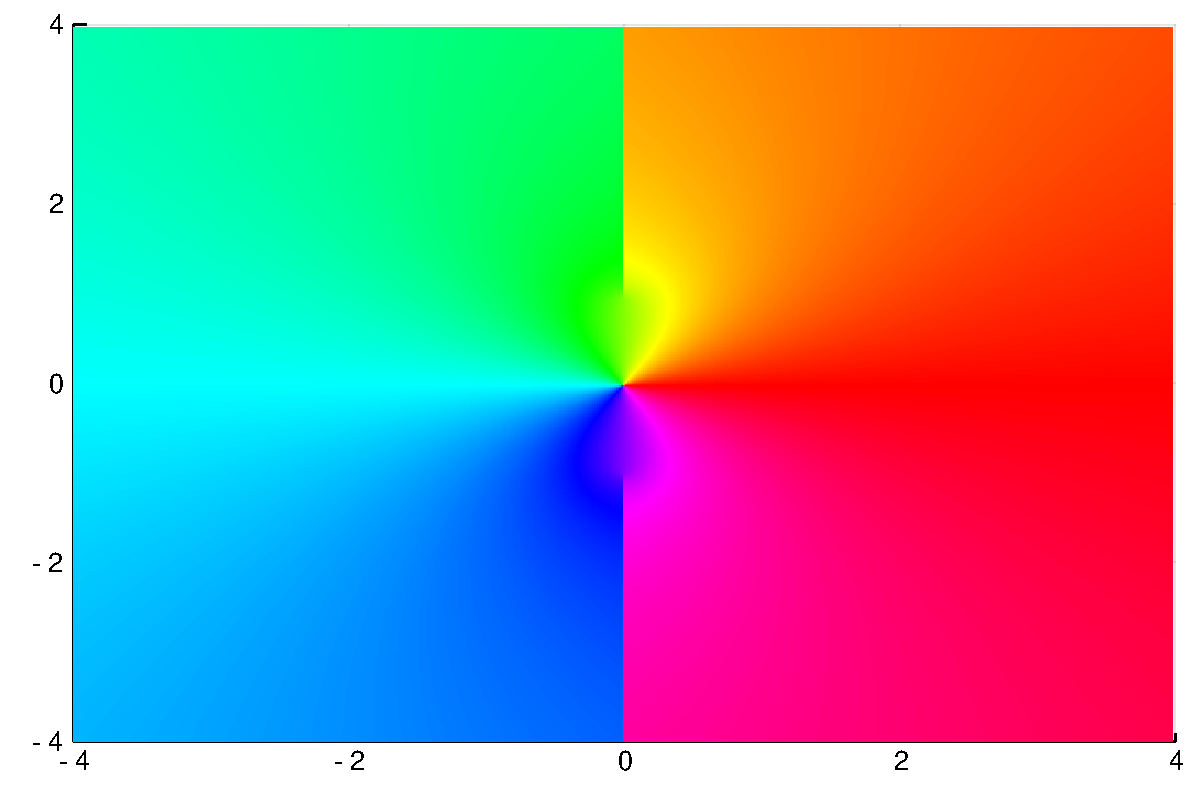
\includegraphics[width=\linewidth]{figures/Lecture1_18_1.pdf}

The following example $\sqrt{z-1} \sqrt{z+1}$ is analytic in ${\mathbb C}\backslash [-1,1]$ and will be returned to:


\begin{lstlisting}
(*@\HLJLnf{phaseplot}@*)(*@\HLJLp{(}@*)(*@\HLJLoB{-}@*)(*@\HLJLnfB{4..4}@*)(*@\HLJLp{,}@*) (*@\HLJLoB{-}@*)(*@\HLJLnfB{4..4}@*)(*@\HLJLp{,}@*) (*@\HLJLn{z}@*) (*@\HLJLoB{->}@*) (*@\HLJLnf{sqrt}@*)(*@\HLJLp{(}@*)(*@\HLJLn{z}@*)(*@\HLJLoB{-}@*)(*@\HLJLni{1}@*)(*@\HLJLp{)}@*)(*@\HLJLnf{sqrt}@*)(*@\HLJLp{(}@*)(*@\HLJLn{z}@*)(*@\HLJLoB{+}@*)(*@\HLJLni{1}@*)(*@\HLJLp{))}@*)
\end{lstlisting}

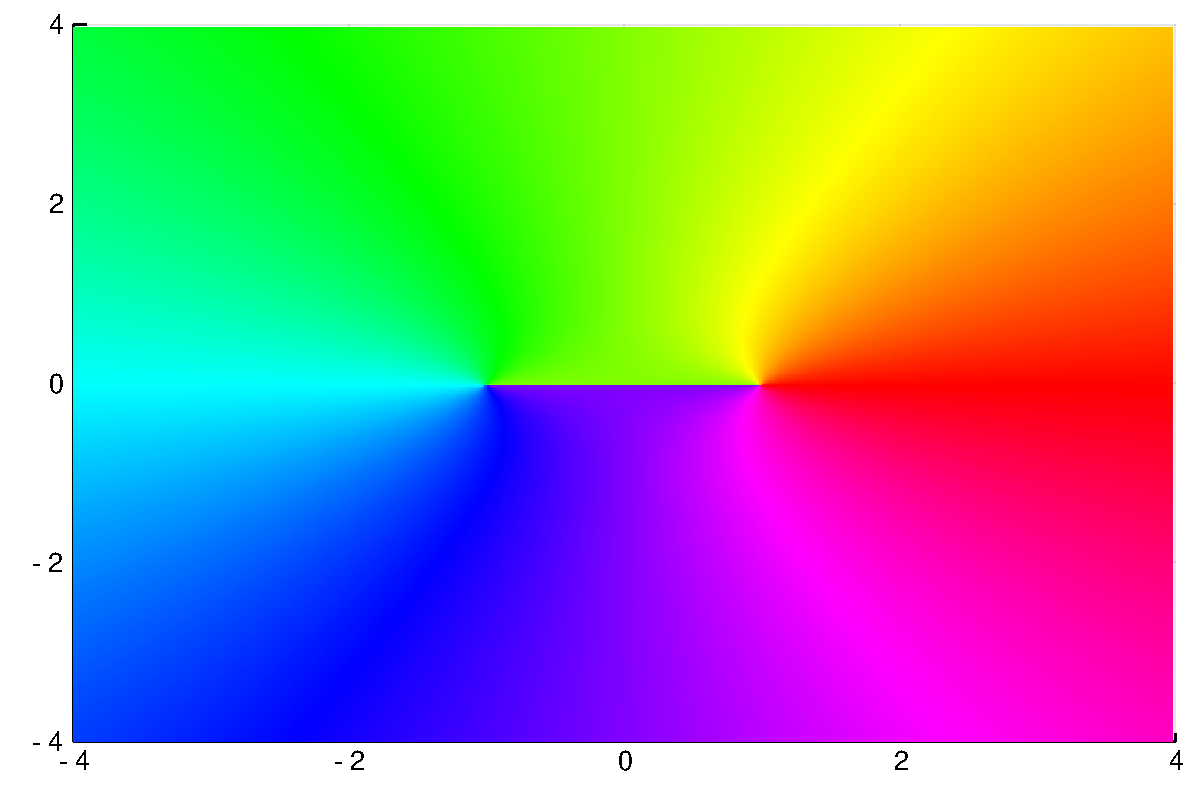
\includegraphics[width=\linewidth]{figures/Lecture1_19_1.pdf}

Here's an example of a closed contour that is not simple:


\begin{lstlisting}
(*@\HLJLn{a}@*)(*@\HLJLp{,}@*)(*@\HLJLn{b}@*) (*@\HLJLoB{=}@*) (*@\HLJLoB{-}@*)(*@\HLJLn{\ensuremath{\pi}}@*)(*@\HLJLp{,}@*) (*@\HLJLn{\ensuremath{\pi}}@*)
(*@\HLJLn{tt}@*) (*@\HLJLoB{=}@*) (*@\HLJLnf{range}@*)(*@\HLJLp{(}@*)(*@\HLJLn{a}@*)(*@\HLJLp{,}@*) (*@\HLJLn{stop}@*)(*@\HLJLoB{=}@*)(*@\HLJLn{b}@*)(*@\HLJLp{,}@*) (*@\HLJLn{length}@*)(*@\HLJLoB{=}@*)(*@\HLJLni{1000}@*)(*@\HLJLp{)}@*)

(*@\HLJLn{\ensuremath{\gamma}}@*) (*@\HLJLoB{=}@*) (*@\HLJLn{t}@*) (*@\HLJLoB{->}@*) (*@\HLJLnf{exp}@*)(*@\HLJLp{(}@*)(*@\HLJLn{im}@*)(*@\HLJLoB{*}@*)(*@\HLJLn{t}@*)(*@\HLJLp{)}@*) (*@\HLJLoB{+}@*)(*@\HLJLnf{exp}@*)(*@\HLJLp{(}@*)(*@\HLJLni{2}@*)(*@\HLJLn{im}@*)(*@\HLJLoB{*}@*)(*@\HLJLn{t}@*)(*@\HLJLp{)}@*)

(*@\HLJLnf{plot}@*)(*@\HLJLp{(}@*)(*@\HLJLn{real}@*)(*@\HLJLoB{.}@*)(*@\HLJLp{(}@*)(*@\HLJLn{\ensuremath{\gamma}}@*)(*@\HLJLoB{.}@*)(*@\HLJLp{(}@*)(*@\HLJLn{tt}@*)(*@\HLJLp{)),}@*) (*@\HLJLn{imag}@*)(*@\HLJLoB{.}@*)(*@\HLJLp{(}@*)(*@\HLJLn{\ensuremath{\gamma}}@*)(*@\HLJLoB{.}@*)(*@\HLJLp{(}@*)(*@\HLJLn{tt}@*)(*@\HLJLp{));}@*) (*@\HLJLn{ratio}@*)(*@\HLJLoB{=}@*)(*@\HLJLnfB{1.0}@*)(*@\HLJLp{,}@*) (*@\HLJLn{legend}@*)(*@\HLJLoB{=}@*)(*@\HLJLkc{false}@*)(*@\HLJLp{,}@*) (*@\HLJLn{arrow}@*)(*@\HLJLoB{=}@*)(*@\HLJLkc{true}@*)(*@\HLJLp{)}@*)
\end{lstlisting}

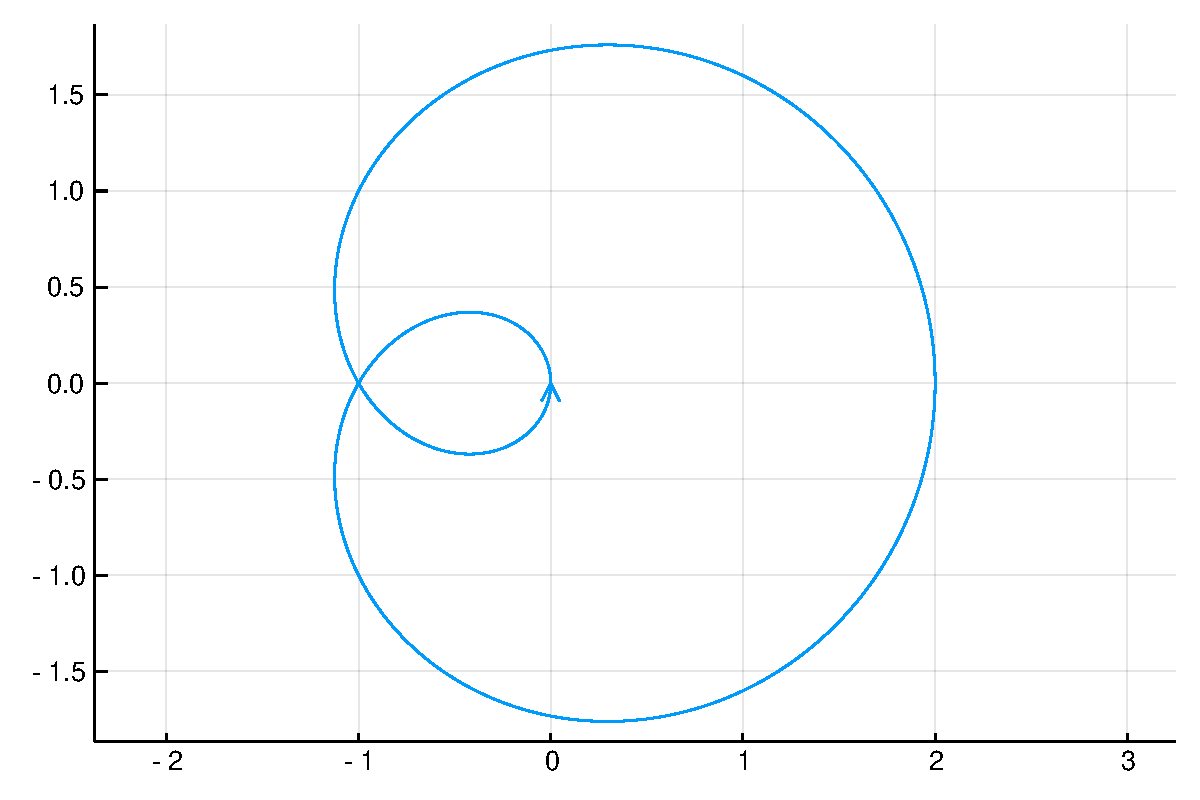
\includegraphics[width=\linewidth]{figures/Lecture1_20_1.pdf}

The notion of integration over a contour in the complex plane  is independent of the notion of holomorphicity. For example, we can happily define the integral for non-holomorphic functions such as $\Re \E^z = \E^x \cos y$:


\begin{lstlisting}
(*@\HLJLn{f}@*) (*@\HLJLoB{=}@*) (*@\HLJLnf{Fun}@*)(*@\HLJLp{(}@*) (*@\HLJLn{z}@*) (*@\HLJLoB{->}@*) (*@\HLJLnf{real}@*)(*@\HLJLp{(}@*)(*@\HLJLnf{exp}@*)(*@\HLJLp{(}@*)(*@\HLJLn{z}@*)(*@\HLJLp{)),}@*) (*@\HLJLnf{Arc}@*)(*@\HLJLp{(}@*)(*@\HLJLnfB{0.}@*)(*@\HLJLp{,}@*)(*@\HLJLnfB{1.}@*)(*@\HLJLp{,(}@*)(*@\HLJLni{0}@*)(*@\HLJLp{,}@*)(*@\HLJLn{\ensuremath{\pi}}@*)(*@\HLJLoB{/}@*)(*@\HLJLni{2}@*)(*@\HLJLp{)))}@*)  (*@\HLJLcs{{\#}}@*) (*@\HLJLcs{Not}@*) (*@\HLJLcs{holomorphic!}@*)

(*@\HLJLnf{plot}@*)(*@\HLJLp{(}@*)(*@\HLJLnf{domain}@*)(*@\HLJLp{(}@*)(*@\HLJLn{f}@*)(*@\HLJLp{);}@*) (*@\HLJLn{legend}@*)(*@\HLJLoB{=}@*)(*@\HLJLkc{false}@*)(*@\HLJLp{,}@*) (*@\HLJLn{ratio}@*)(*@\HLJLoB{=}@*)(*@\HLJLnfB{1.0}@*)(*@\HLJLp{,}@*) (*@\HLJLn{arrow}@*)(*@\HLJLoB{=}@*)(*@\HLJLkc{true}@*)(*@\HLJLp{)}@*)
\end{lstlisting}

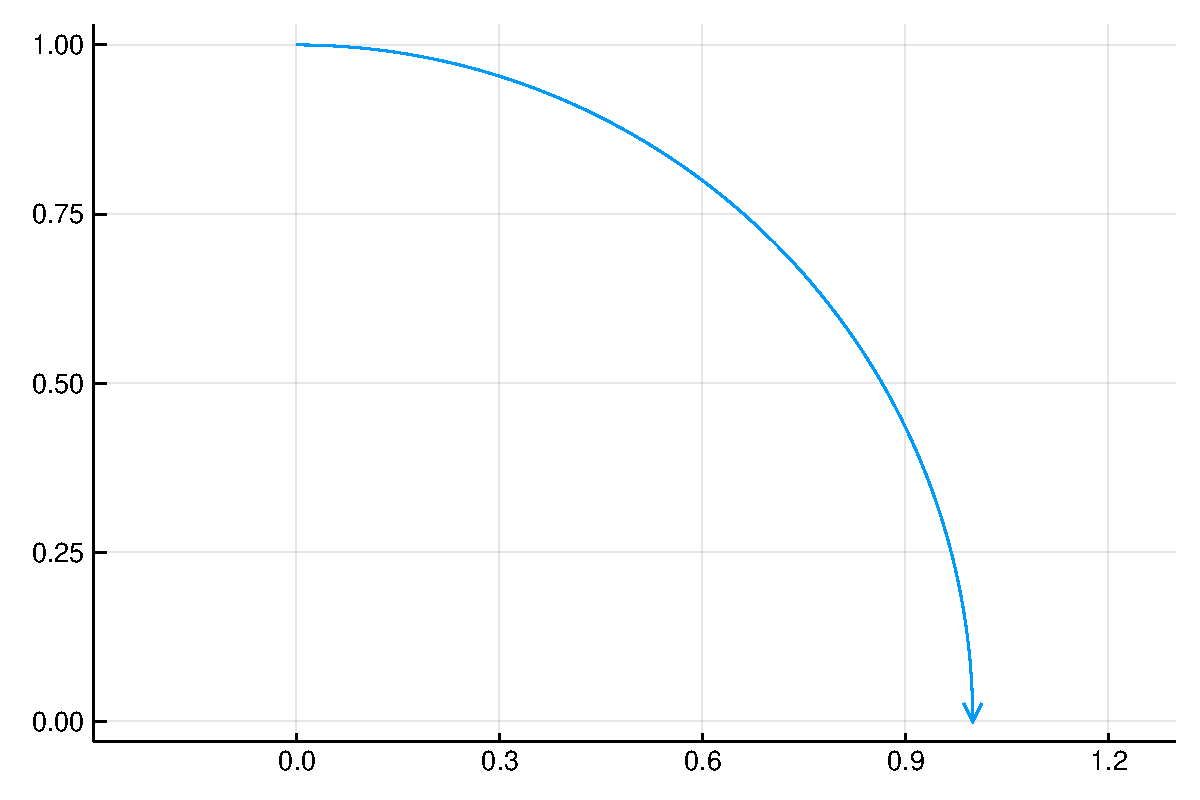
\includegraphics[width=\linewidth]{figures/Lecture1_21_1.pdf}

\begin{lstlisting}
(*@\HLJLnf{sum}@*)(*@\HLJLp{(}@*)(*@\HLJLn{f}@*)(*@\HLJLp{)}@*)  (*@\HLJLcs{{\#}}@*) (*@\HLJLcs{this}@*) (*@\HLJLcs{means}@*) (*@\HLJLcs{contour}@*) (*@\HLJLcs{integral}@*)
\end{lstlisting}

\begin{lstlisting}
-1.2485382363935424 + 1.949326343919058im
\end{lstlisting}


This is defined in terms of a parameterization, and so the following real integral gives the same result:


\begin{lstlisting}
(*@\HLJLn{g}@*) (*@\HLJLoB{=}@*) (*@\HLJLn{im}@*)(*@\HLJLoB{*}@*)(*@\HLJLnf{Fun}@*)(*@\HLJLp{(}@*)(*@\HLJLn{t}@*)(*@\HLJLoB{->}@*) (*@\HLJLnf{f}@*)(*@\HLJLp{(}@*)(*@\HLJLnf{exp}@*)(*@\HLJLp{(}@*)(*@\HLJLn{im}@*)(*@\HLJLoB{*}@*)(*@\HLJLn{t}@*)(*@\HLJLp{))}@*)(*@\HLJLoB{*}@*)(*@\HLJLnf{exp}@*)(*@\HLJLp{(}@*)(*@\HLJLn{im}@*)(*@\HLJLoB{*}@*)(*@\HLJLn{t}@*)(*@\HLJLp{),}@*) (*@\HLJLni{0}@*) (*@\HLJLoB{..}@*) (*@\HLJLn{\ensuremath{\pi}}@*)(*@\HLJLoB{/}@*)(*@\HLJLni{2}@*)(*@\HLJLp{)}@*)
(*@\HLJLnf{sum}@*)(*@\HLJLp{(}@*) (*@\HLJLn{g}@*) (*@\HLJLp{)}@*)  (*@\HLJLcs{{\#}}@*) (*@\HLJLcs{this}@*) (*@\HLJLcs{is}@*) (*@\HLJLcs{standard}@*) (*@\HLJLcs{integral}@*)
\end{lstlisting}

\begin{lstlisting}
-1.2485382363935429 + 1.9493263439190578im
\end{lstlisting}


The following show that the contour of integration does not affect the integral for holomorphic functions:


\begin{lstlisting}
(*@\HLJLn{f}@*) (*@\HLJLoB{=}@*) (*@\HLJLnf{Fun}@*)(*@\HLJLp{(}@*) (*@\HLJLn{z}@*) (*@\HLJLoB{->}@*) (*@\HLJLnf{exp}@*)(*@\HLJLp{(}@*)(*@\HLJLn{z}@*)(*@\HLJLp{),}@*) (*@\HLJLnf{Arc}@*)(*@\HLJLp{(}@*)(*@\HLJLnfB{0.}@*)(*@\HLJLp{,}@*)(*@\HLJLnfB{1.}@*)(*@\HLJLp{,(}@*)(*@\HLJLni{0}@*)(*@\HLJLp{,}@*)(*@\HLJLn{\ensuremath{\pi}}@*)(*@\HLJLoB{/}@*)(*@\HLJLni{2}@*)(*@\HLJLp{)))}@*) (*@\HLJLcs{{\#}integrate}@*) (*@\HLJLcs{over}@*) (*@\HLJLcs{an}@*) (*@\HLJLcs{arc}@*)
(*@\HLJLnf{sum}@*)(*@\HLJLp{(}@*)(*@\HLJLn{f}@*)(*@\HLJLp{)}@*)  (*@\HLJLp{,}@*) (*@\HLJLnf{f}@*)(*@\HLJLp{(}@*)(*@\HLJLn{im}@*)(*@\HLJLp{)}@*)(*@\HLJLoB{-}@*)(*@\HLJLnf{f}@*)(*@\HLJLp{(}@*)(*@\HLJLni{1}@*)(*@\HLJLp{)}@*)
\end{lstlisting}

\begin{lstlisting}
(-2.1779795225909058 + 0.8414709848078968im, -2.177979522590906 + 0.8414709
848078968im)
\end{lstlisting}


\begin{lstlisting}
(*@\HLJLn{f}@*) (*@\HLJLoB{=}@*) (*@\HLJLnf{Fun}@*)(*@\HLJLp{(}@*) (*@\HLJLn{z}@*) (*@\HLJLoB{->}@*) (*@\HLJLnf{exp}@*)(*@\HLJLp{(}@*)(*@\HLJLn{z}@*)(*@\HLJLp{),}@*) (*@\HLJLnf{Segment}@*)(*@\HLJLp{(}@*)(*@\HLJLni{1}@*)(*@\HLJLp{,}@*)(*@\HLJLn{im}@*)(*@\HLJLp{))}@*) (*@\HLJLcs{{\#}}@*) (*@\HLJLcs{integrate}@*) (*@\HLJLcs{over}@*) (*@\HLJLcs{a}@*) (*@\HLJLcs{line}@*) (*@\HLJLcs{segment}@*)
(*@\HLJLnf{sum}@*)(*@\HLJLp{(}@*)(*@\HLJLn{f}@*)(*@\HLJLp{)}@*)  (*@\HLJLp{,}@*) (*@\HLJLnf{f}@*)(*@\HLJLp{(}@*)(*@\HLJLn{im}@*)(*@\HLJLp{)}@*)(*@\HLJLoB{-}@*)(*@\HLJLnf{f}@*)(*@\HLJLp{(}@*)(*@\HLJLni{1}@*)(*@\HLJLp{)}@*)
\end{lstlisting}

\begin{lstlisting}
(-2.1779795225909053 + 0.8414709848078966im, -2.177979522590907 + 0.8414709
848078968im)
\end{lstlisting}


The following demonstrates Cauchy's theorem, integration over a closed contour equals zero:


\begin{lstlisting}
(*@\HLJLn{f}@*) (*@\HLJLoB{=}@*) (*@\HLJLnf{Fun}@*)(*@\HLJLp{(}@*) (*@\HLJLn{z}@*) (*@\HLJLoB{->}@*) (*@\HLJLnf{exp}@*)(*@\HLJLp{(}@*)(*@\HLJLn{z}@*)(*@\HLJLp{),}@*) (*@\HLJLnf{Circle}@*)(*@\HLJLp{())}@*)  (*@\HLJLcs{{\#}}@*)  (*@\HLJLcs{Holomorphic!}@*)
(*@\HLJLnf{sum}@*)(*@\HLJLp{(}@*)(*@\HLJLn{f}@*)(*@\HLJLp{)}@*)
\end{lstlisting}

\begin{lstlisting}
2.9644937254112756e-17 - 1.4872544363724962e-16im
\end{lstlisting}


If \texttt{f} is not holomorphic, it doesn't apply:


\begin{lstlisting}
(*@\HLJLn{f}@*) (*@\HLJLoB{=}@*) (*@\HLJLnf{Fun}@*)(*@\HLJLp{(}@*) (*@\HLJLn{z}@*) (*@\HLJLoB{->}@*) (*@\HLJLnf{exp}@*)(*@\HLJLp{(}@*)(*@\HLJLn{z}@*)(*@\HLJLp{)}@*)(*@\HLJLoB{/}@*)(*@\HLJLn{z}@*)(*@\HLJLp{,}@*) (*@\HLJLnf{Circle}@*)(*@\HLJLp{())}@*)  (*@\HLJLcs{{\#}}@*) (*@\HLJLcs{Not}@*) (*@\HLJLcs{holomorphic}@*) (*@\HLJLcs{at}@*) (*@\HLJLcs{zero}@*)
(*@\HLJLnf{sum}@*)(*@\HLJLp{(}@*)(*@\HLJLn{f}@*)(*@\HLJLp{)}@*)
\end{lstlisting}

\begin{lstlisting}
-9.96316757509274e-16 + 6.283185307179588im
\end{lstlisting}


\begin{lstlisting}
(*@\HLJLn{f}@*) (*@\HLJLoB{=}@*) (*@\HLJLnf{Fun}@*)(*@\HLJLp{(}@*) (*@\HLJLn{z}@*) (*@\HLJLoB{->}@*) (*@\HLJLnf{real}@*)(*@\HLJLp{(}@*)(*@\HLJLnf{exp}@*)(*@\HLJLp{(}@*)(*@\HLJLn{z}@*)(*@\HLJLp{)),}@*) (*@\HLJLnf{Circle}@*)(*@\HLJLp{())}@*)  (*@\HLJLcs{{\#}}@*) (*@\HLJLcs{Not}@*) (*@\HLJLcs{holomorphic}@*) (*@\HLJLcs{anywhere!}@*)
(*@\HLJLnf{sum}@*)(*@\HLJLp{(}@*)(*@\HLJLn{f}@*)(*@\HLJLp{)}@*)
\end{lstlisting}

\begin{lstlisting}
-3.3420237696193494e-16 + 3.141592653589793im
\end{lstlisting}


We can test contour deformation experimentally: in the following, the  integral (implemented as \texttt{sum}) over two different contours returns the  same value (up to numerical precision)


\begin{lstlisting}
(*@\HLJLn{f}@*) (*@\HLJLoB{=}@*) (*@\HLJLnf{Fun}@*)(*@\HLJLp{(}@*) (*@\HLJLn{z}@*) (*@\HLJLoB{->}@*) (*@\HLJLnf{exp}@*)(*@\HLJLp{(}@*)(*@\HLJLn{z}@*)(*@\HLJLp{),}@*) (*@\HLJLnf{Arc}@*)(*@\HLJLp{(}@*)(*@\HLJLnfB{0.}@*)(*@\HLJLp{,}@*)(*@\HLJLnfB{1.}@*)(*@\HLJLp{,(}@*)(*@\HLJLni{0}@*)(*@\HLJLp{,}@*)(*@\HLJLn{\ensuremath{\pi}}@*)(*@\HLJLoB{/}@*)(*@\HLJLni{2}@*)(*@\HLJLp{)))}@*)  (*@\HLJLcs{{\#}}@*) (*@\HLJLcs{Holomorphic!}@*)
(*@\HLJLn{fs}@*) (*@\HLJLoB{=}@*) (*@\HLJLnf{Fun}@*)(*@\HLJLp{(}@*) (*@\HLJLn{z}@*) (*@\HLJLoB{->}@*) (*@\HLJLnf{exp}@*)(*@\HLJLp{(}@*)(*@\HLJLn{z}@*)(*@\HLJLp{),}@*) (*@\HLJLnf{Segment}@*)(*@\HLJLp{(}@*)(*@\HLJLni{1}@*)(*@\HLJLp{,}@*)(*@\HLJLn{im}@*)(*@\HLJLp{))}@*)  (*@\HLJLcs{{\#}}@*) (*@\HLJLcs{Holomorphic!}@*)

(*@\HLJLnf{sum}@*)(*@\HLJLp{(}@*)(*@\HLJLn{f}@*)(*@\HLJLp{)}@*)  (*@\HLJLp{,}@*) (*@\HLJLnf{sum}@*)(*@\HLJLp{(}@*)(*@\HLJLn{fs}@*)(*@\HLJLp{)}@*)
\end{lstlisting}

\begin{lstlisting}
(-2.1779795225909058 + 0.8414709848078968im, -2.1779795225909053 + 0.841470
9848078966im)
\end{lstlisting}


Here is a depection of the two contours:


\begin{lstlisting}
(*@\HLJLnf{plot}@*)(*@\HLJLp{(}@*)(*@\HLJLnf{domain}@*)(*@\HLJLp{(}@*)(*@\HLJLn{f}@*)(*@\HLJLp{);}@*) (*@\HLJLn{ratio}@*)(*@\HLJLoB{=}@*)(*@\HLJLnfB{1.0}@*)(*@\HLJLp{,}@*) (*@\HLJLn{legend}@*)(*@\HLJLoB{=}@*)(*@\HLJLkc{false}@*)(*@\HLJLp{,}@*) (*@\HLJLn{arrow}@*)(*@\HLJLoB{=}@*)(*@\HLJLkc{true}@*)(*@\HLJLp{)}@*)
(*@\HLJLnf{plot!}@*)(*@\HLJLp{(}@*)(*@\HLJLnf{domain}@*)(*@\HLJLp{(}@*)(*@\HLJLn{fs}@*)(*@\HLJLp{),}@*) (*@\HLJLn{arrow}@*)(*@\HLJLoB{=}@*)(*@\HLJLkc{true}@*)(*@\HLJLp{)}@*)
\end{lstlisting}

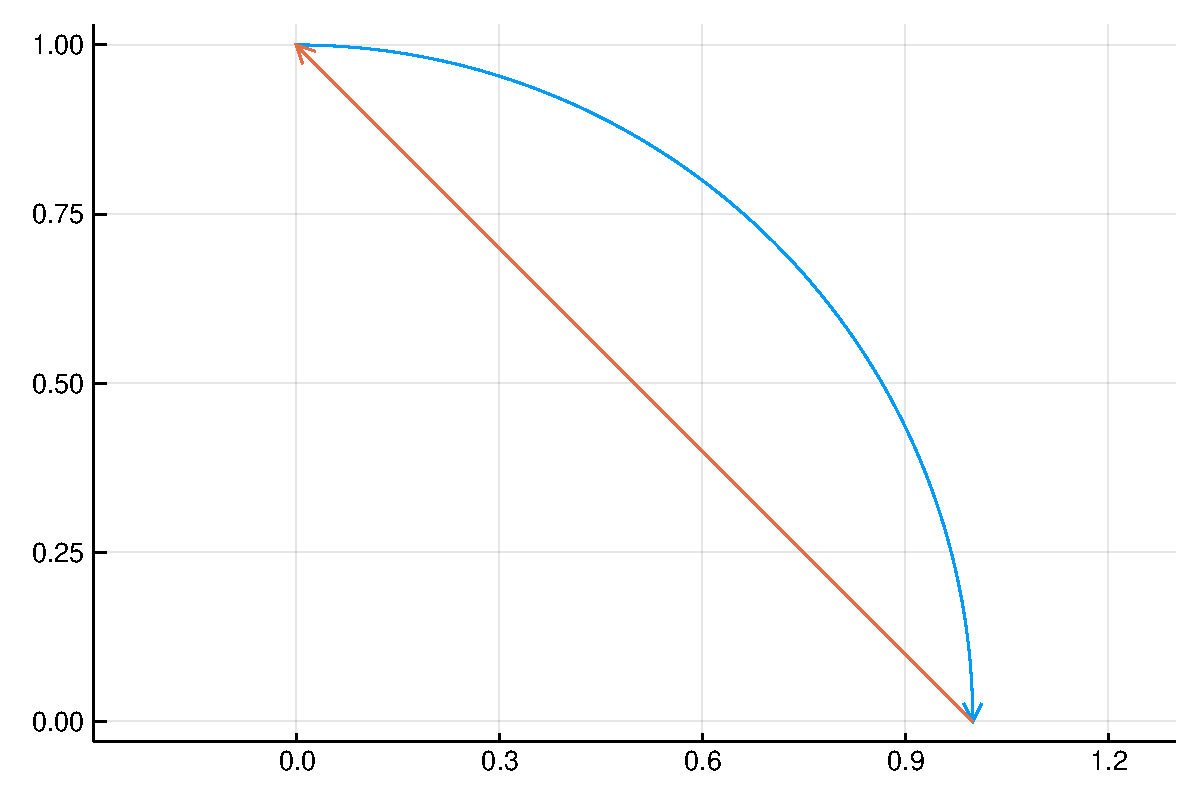
\includegraphics[width=\linewidth]{figures/Lecture1_30_1.pdf}


\end{document}
